\chapter{Locomotion in Hydrodynamic Environments}

\section{Motivation}

We live on a planet that is covered mostly by water, in which a wide variety of
creatures use swimming as their primary form of locomotion.  There are
an astonishing variety of body shapes and patterns of motion that are used
by swimmers across the animal kingdom.  Some of the many creature swimming
patterns from nature include using thrust from a tail, moving an elongated
body sinusoidally, using paddle-like motions of flippers, kicking with legs,
and gentle bird-like flapping of fins.  Our research goal is to develop a
general platform for finding efficient swimming motion for a given creature
body shape.  There are a number of application areas that can benefit from
realistic swimming simulation, including feature film
animation~\cite{stanton2003finding}, biological investigation of swimming
mechanics~\cite{kern2006simulations,shirgaonkar2008hydrodynamics},
locomotion of user-created creatures in video games~\cite{hecker2008real},
and the invention of new modes of propulsion for underwater
vehicles~\cite{barrett2002optimal}.

Today, most scientific models for swimming motion are customized to specific
species with predefined locomotion patterns
\cite{shirgaonkar2008hydrodynamics}. These models are
highly accurate but are difficult to generalize to a variety of creatures.
The existing 3D swimming animations, on the other hand, demonstrate a
lifelike underwater ecosystem with rich variety of creatures. However, their motions are typically animated
manually or based on simplified physical models. Having a generic set of
tools that can produce physically realistic aquatic motion for a wide array
of creatures is challenging and has not been shown in previous work.

At the heart of synthesizing realistic aquatic locomotion lies the
problems of simulation and control. Solving these two problems
simultaneously under hydrodynamics presents some unique
challenges. First, the relation between the movement of the aquatic
animal and the forces exerted by surrounding fluid is extremely
complex. Thus it is difficult to solve using an optimization approach. Any small
changes in undulation or flapping gait can result in drastically
different control strategies. In addition, the morphology of aquatic
animals is astonishingly diverse and results in fundamentally
different locomotion mechanisms. Designing control strategies based on
ad-hoc observation or careful tuning of parameters would be extraordinarily difficult to generalize to the vast biodiversity found in nature.

This chapter describes a complete system for controlling a wide variety of
aquatic animals in a simulated fluid environment. Our goal is a system
that balances between physical realism and generality. Given an aquatic
animal that is represented by an articulated rigid body system, our system
can automatically find the optimal locomotion in a
hydrodynamically-coupled environment. Our system does not require any
prior knowledge of the animal's behavior and minimizes the effort of
manually tuning the physical and control parameters.

The system consists of two main components: simulating motion and
optimizing control strategies. We simulate articulated rigid bodies
submerged in invisid, incompressible fluid governed by the Navier-Stokes
equations. The animal can exert torques to exercise each actuated
joint. Through accurate two-way coupling of the rigid bodies and the
fluid, the joint motion will lead to \emph{some} locomotion in the
fluid, but purposeful and balanced locomotion requires careful
coordination and synchronization among those actuated joints.  The
second component provides an automatic way to discover joint motion
that achieves a desired goal in locomotion (i.e. a joint motion that
yields the fastest or the most energy efficient locomotion).  We
employ an optimization technique called Covariance Matrix Adaptation
(CMA) to explore the domain of possible joint trajectories.

We evaluate our system by demonstrating optimized swimming gaits for a
wider variety of aquatic animals and swimming strategies, including
clownfish, eels, sea turtles, frogs, manta rays and some imaginary
creatures. In addition, we compare the swimming motion in a Navier-Stokes
fluid with motion in a simplified fluid. Our results show that these
motions can differ dramatically depending on which fluid model is used.

\section{Swimming Simulation}

We simulate fluids by solving the Navier-Stokes equations on a MAC grid
and we simulate the articulated rigid body using generalized coordinates.
We modify the projection step of the fluid solver to take into
consideration the dynamics of the articulated figure.

\subsection{Fluid Simulation}

We simulate fluid using the inviscid, incompressible fluid equations
(sometimes called the Euler equations):
\begin{displaymath}
 \nabla\cdot\mathbf{u}=0
\end{displaymath}
\begin{displaymath}
 \mathbf{u}_t=-(\mathbf{u}\cdot\nabla\mathbf{u})-\frac{1}{\rho}\nabla
 p+\mathbf{f}
\end{displaymath}
where $\mathbf{u}=(u,v,w)$ is the velocity of fluids, $p$ is the pressure,
$\rho$ is the density and $\mathbf{f}$ accounts for the external body
forces.  We do not include a viscous term because such effects are
negligable for the motion of the large animals in our examples.  If we
were studying swimming of millimeter sized creatures, however,
incorporating viscous effects would be mandatory.

The standard way to solve the above equations on a MAC grid can be described in following two steps. First, we calculate an intermediate velocity field $\mathbf{u}^*$ by only considering the convection $\mathbf{u}\cdot\nabla\mathbf{u}$ and the body force $\mathbf{f}$:
\begin{equation}
 \mathbf{u}^*=\textrm{SL}(\mathbf{u}^n,\Delta t)+\Delta t\mathbf{f}
\label{eq:sl}
\end{equation}
where $\mathbf{u}^n$ is the velocity at $n^{th}$ time step.
We use the Semi-Lagrangian method \cite{stam99stablefluids} to integrate the convection term and apply BFECC \cite{kim06advectionswith} to reduce the numerical dissipation.

Next, we solve the following Poisson equation with Neumann boundary conditions $\mathbf{u}\cdot\mathbf{n}=\mathbf{u}_{solid}\cdot\mathbf{n}$ at the solid boundary and Dirichlet
boundary conditions $p = 0$ at the free surface. Then we project the intermediate velocity field to ensure the incompressibility condition.
\begin{equation}
\label{eq:poissonEqu}
 \nabla^2 p=\frac{\rho}{\Delta t}\nabla\cdot\mathbf{u}^*
\end{equation}
\begin{equation}
\label{eq:projection}
 \mathbf{u}^{n+1}=\mathbf{u}^*-\frac{\Delta t}{\rho}\nabla p
\end{equation}
In this work, we modify the second step ((\ref{eq:poissonEqu}) and (\ref{eq:projection})) to take into account the interaction between the fluid and the articulated rigid bodies.

\subsection{Articulated Rigid Body Simulation}
In this section, we will describe the numerical techniques that we use to move the body parts of an articulated figure. Later, in Section 4, we will describe the optimization technique that we use to discover efficient swimming gaits.

The dynamic equations of an articulated rigid body in generalized coordinates can be expressed as follows.
\begin{equation}
\label{eq:dynamics}
\mathbf{M}(\mathbf{q})\mathbf{\ddot{q}}+\mathbf{C}(\mathbf{q},\mathbf{\dot{q}})=\mathbf{\tau}_{int}+\mathbf{\tau}_{ext}
\end{equation}
where $\mathbf{q}$, $\mathbf{\dot{q}}$ and $\mathbf{\ddot{q}}$ are vectors of positions, velocities and accelerations of joint degrees of freedom respectively. $\mathbf{M}(\mathbf{q})$ is the mass matrix and $\mathbf{C}(\mathbf{q},\mathbf{\dot{q}})$ accounts for the Coriolis and Centrifugal force. $\mathbf{\tau}_{int}$ and $\mathbf{\tau}_{ext}$ are internal and external generalized forces.

Given the current state $\mathbf{q}^n$ and $\mathbf{\dot{q}}^n$, we can
evaluate $\mathbf{M}$ and $\mathbf{C}$ of (\ref{eq:dynamics}). For the
external forces $\mathbf{\tau}_{ext}$, we consider the
fluid pressure force. We make use of the modified PD controller of Tan et al. \cite{Tan11SPD} in order to calculate the internal force $\mathbf{\tau}_{int}$ that closely tracks a reference trajectory. Although the details of this method can be found in \cite{Tan11SPD}, we include an overview of this method below. The reference swimming trajectory is computed by an optimization
process described in Section 4. Once we know both the external and
internal forces, we can solve the acceleration $\mathbf{\ddot{q}}^n$ and
advance to the next time step via explicit Euler integration.

\paragraph {Modified Proportional-Derivative Controller} In computer
animation, a PD servo (\ref{eq:pd2}) provides a simple framework to
compute control forces for tracking a kinematic state of a joint
trajectory:
\begin{equation}
\label{eq:pd2}
\tau^n=-k_p(q^n-\bar{q}^n)-k_d\dot{q}^n
\end{equation}
where $k_p$ and $k_d$ are the gain and damping coefficient. In general,
high gain PD servos result in small simulation time steps in order to
maintain stability.

The aquatic creatures in this work require high gain PD servos to track the desired swimming gait closely against strong fluid pressure. However, we cannot reduce the time step to accommodate stability due to the time-consuming fluid simulation. To achieve these two conflicting goals, large time steps and high gains, we modify the PD controller as follows. Instead of using the current state $q^n$ and $\dot{q}^n$ to compute the control force, we compute the control forces using the state at next time step $q^{n+1}$ and $\dot{q}^{n+1}$:
\begin{equation} \label{eq:pd3}
\tau^n=-k_p(q^{n+1}-\bar{q}^{n+1})-k_d\dot{q}^{n+1}
\end{equation}

eq. (\ref{eq:pd3}) can be linearized at $q^n$ and $\dot{q}^n$ as:
\begin{displaymath}
\tau^n=-k_p(q^n+\Delta t\dot{q}^n-\bar{q}^{n+1})-k_d(\dot{q}^n+\Delta t\ddot{q}^n)
\end{displaymath}

Applying the modified PD controller to the articulated rigid body simulation with multiple degrees of freedom, we solve the acceleration as
\begin{displaymath}
\label{eq:modifiedDynamics}
\mathbf{\ddot{q}}^n=(\mathbf{M}+\mathbf{K}_d\Delta t)^{-1}(-\mathbf{C}-\mathbf{K}_p(\mathbf{q}^n+\mathbf{\dot{q}}^n\Delta t-\bar{\mathbf{q}}^{n+1})-\mathbf{K}_d\mathbf{\dot{q}}^n+\mathbf{\tau}_{ext})
\end{displaymath}
where both $\mathbf{K}_p$ and $\mathbf{K}_d$ are diagonal matrices that indicate the gains and damping coefficients.

\subsection{Two-way Coupling Between Fluids and Articulated Rigid Bodies}
The two-way coupling between the incompressible fluid and the articulated figures should satisfy following three conditions.
\begin{enumerate}
\item The normal velocity at the interface between the fluids and the
articulated rigid bodies should agree with each other.
\item The motion of the articulated rigid body resulting from the fluid
pressure force must be consistent with the Lagrangian equations of motion.
\item The fluid should be incompressible.
\end{enumerate}

Two-way coupling is ensured by having the fluid exerting pressure forces
on the rigid bodies, while at the same time the motion of the rigid bodies
affects the pressure distribution of the fluid.

Our simultaneous two-way coupling technique is inspired by Klingner et al.
\cite{klingner2006mesh} since we both start from the acceleration at
cell faces.  Their method uses a tetrahedral mesh to represent the fluid,
and their rigid bodies are in Cartesian space.  Our simulator uses a
regular MAC grid and we couple this fluid with articulated figures that
are described in generalized coordinates.  Similar to Klingner et
al.~\cite{klingner2006mesh}, we split the coupling into two steps
(Figure~\ref{fig:graph}). In the first step, the two systems are solved
independently ignoring the pressure. The fluid solver calculates the
intermediate velocity field $\mathbf{u}^*$ using (\ref{eq:sl}). The articulated
rigid body solver determines the acceleration $\mathbf{\ddot{q}}$ without
external pressure forces and calculates the intermediate velocity
$\mathbf{\dot{q}}^*$.

\begin{figure}[t]
\centering
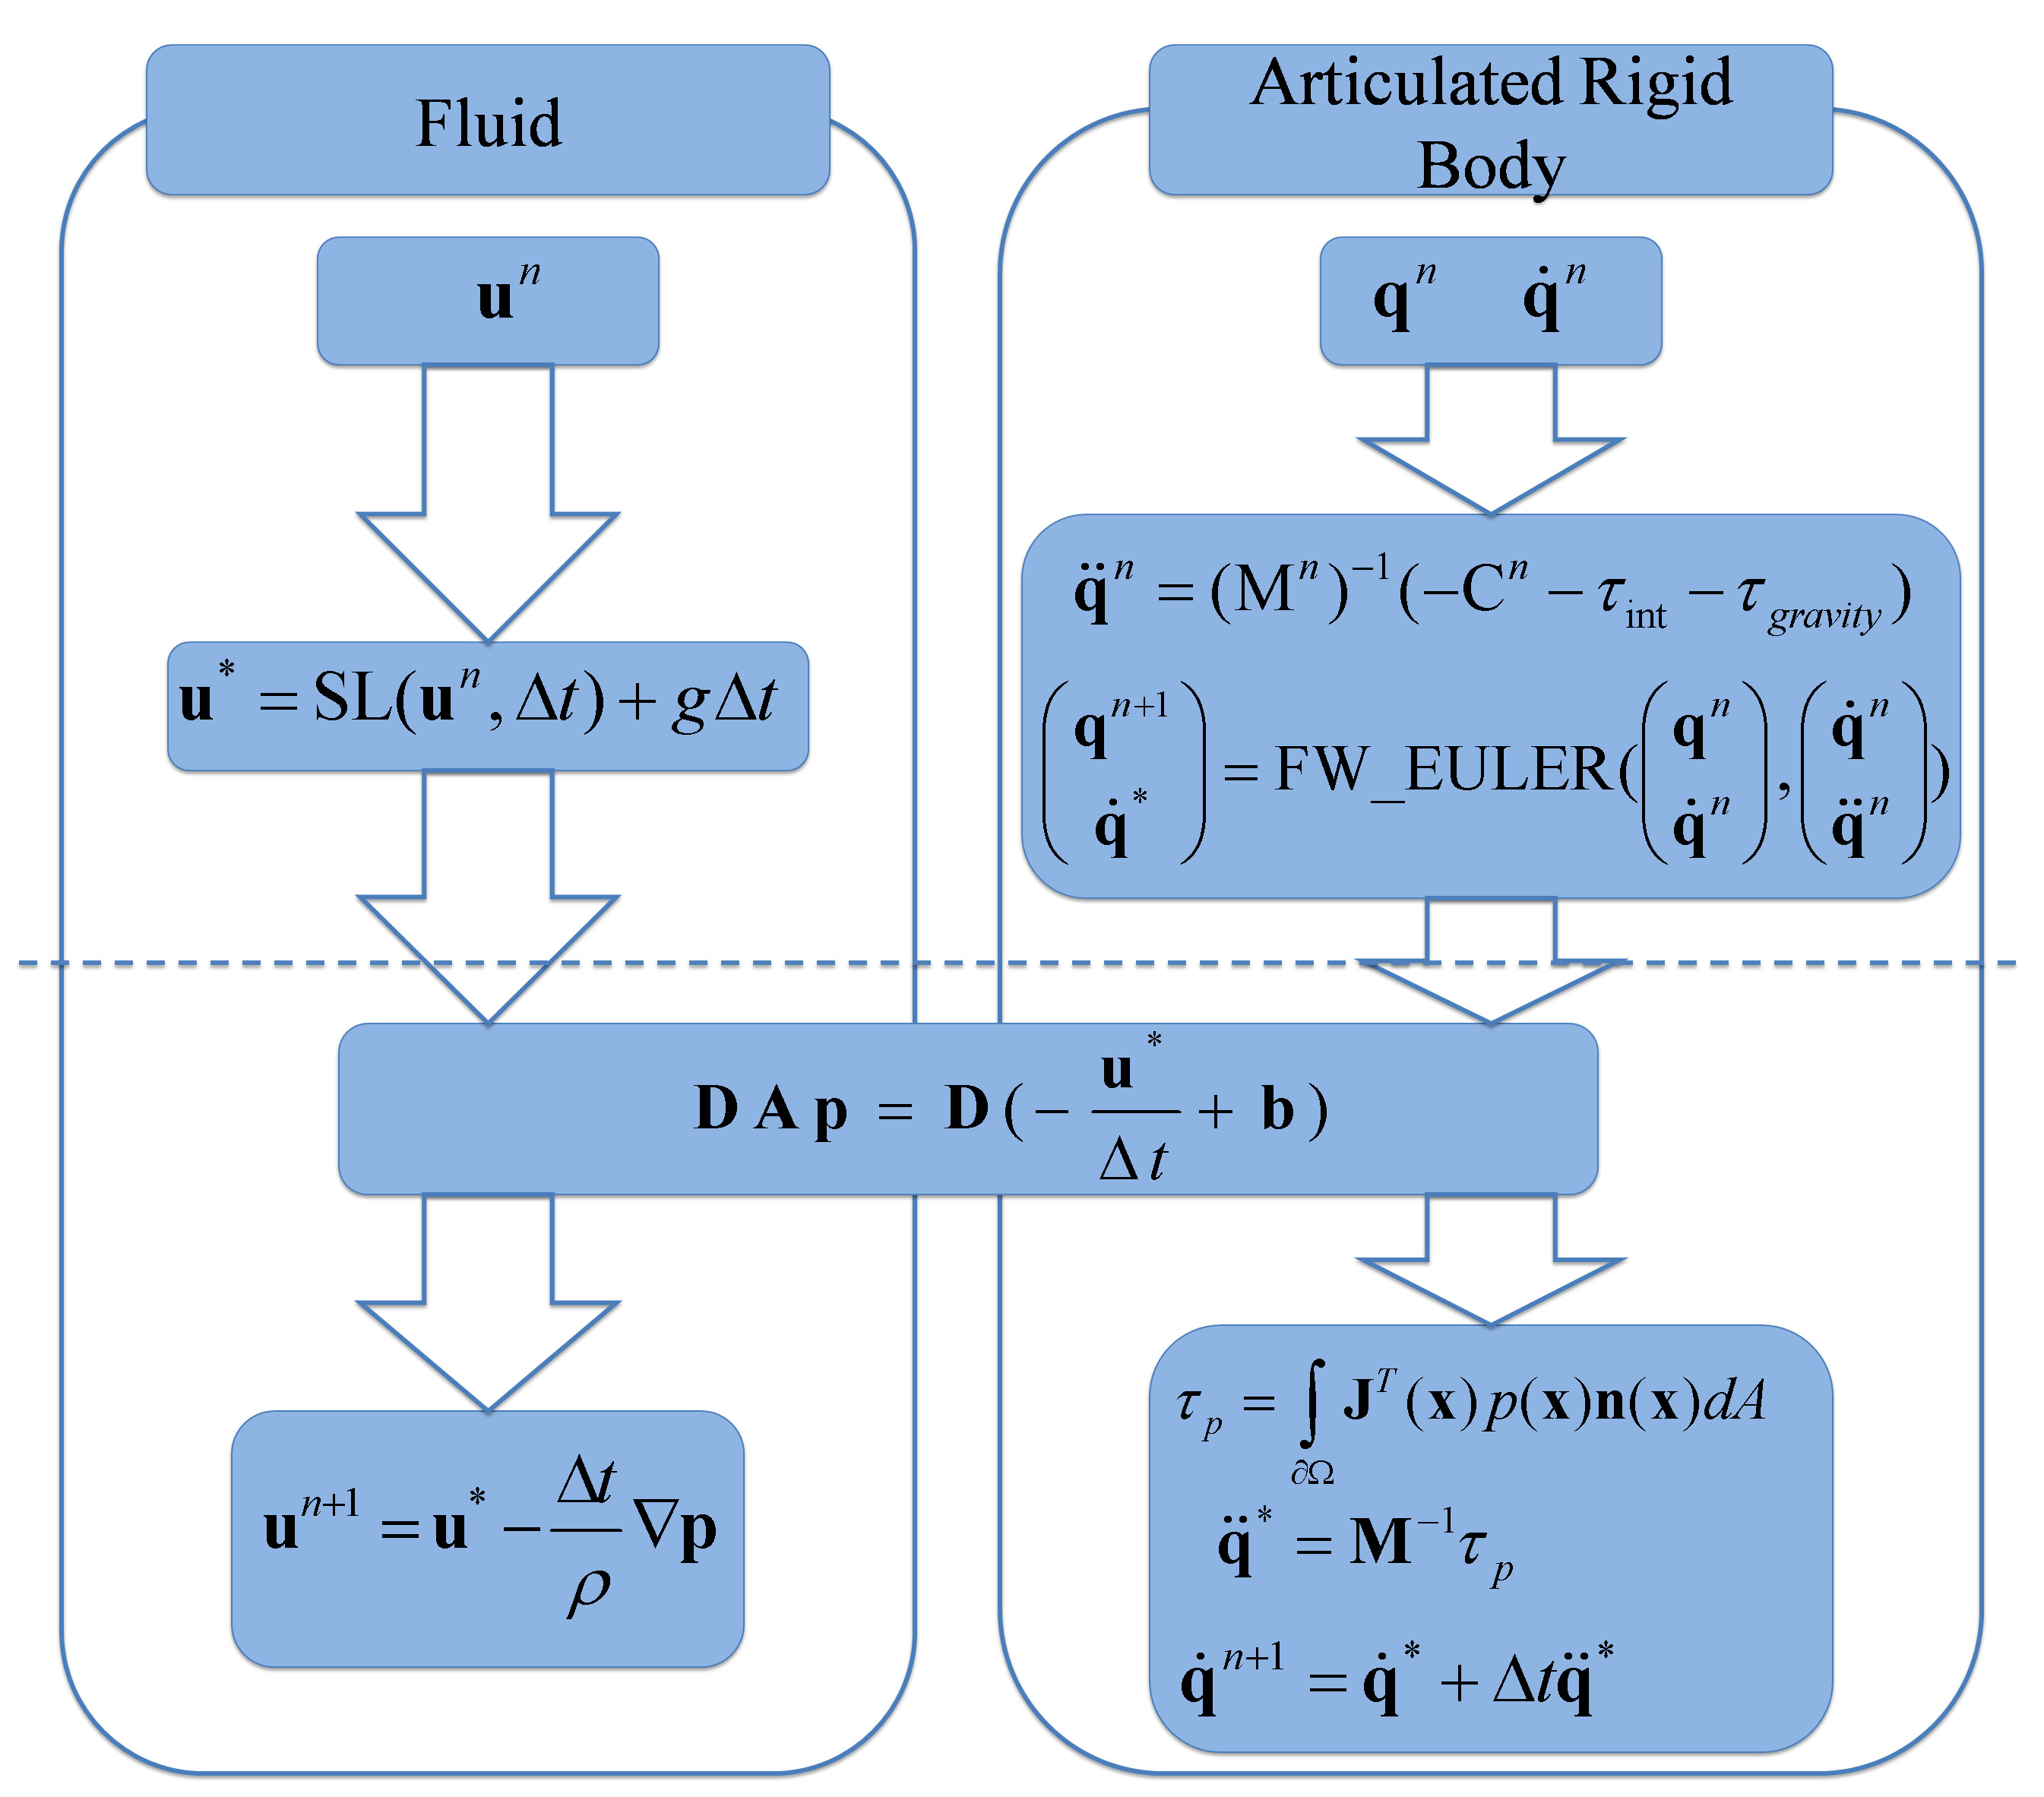
\includegraphics[width=3in]{figures/CouplingProcess.eps}
\caption{The computational steps for simultaneous coupling between fluids and articulated rigid bodies.}
\label{fig:graph}
\end{figure}

In the second step, we consider the motion of the two systems together so
that they will satisfy all above three conditions. We first voxelize the
body segments of the articulated figure (represented by water-tight
polygon meshes) onto the MAC grid and we mark those cells inside the body
segments as SOLID. For two-way coupling, we are particularly interested in
the faces between a SOLID cell and a FLUID cell (defined as \emph{coupled
faces}). The velocity at a coupled face can be expressed in generalized
coordinates by the Jacobian of the articulated rigid body and the joint
velocity:
\begin{displaymath}
\mathbf{u}^*_{solid}=\mathbf{J}\mathbf{\dot{q}}^*
\end{displaymath}
where $\mathbf{J}$ is the $3\times m$ ($m$ is the number of degrees of freedom) Jacobian matrix
\begin{displaymath}
\mathbf{J}=
\left( \begin{array}{cccc}
\frac{\partial x}{\partial q_1} & \frac{\partial x}{\partial q_2} & \ldots & \frac{\partial x}{\partial q_m} \\
\frac{\partial y}{\partial q_1} & \frac{\partial y}{\partial q_2} & \ldots & \frac{\partial y}{\partial q_m} \\
\frac{\partial z}{\partial q_1} & \frac{\partial z}{\partial q_2} & \ldots & \frac{\partial z}{\partial q_m}
\end{array} \right)
\end{displaymath}

Now consider the effect of the pressure field, which exerts forces and
applies accelerations along the face normals $\mathbf{n}$. If a face is
shared by two FLUID cells, the acceleration is
$\frac{1}{\rho}\nabla\mathbf{p}\cdot\mathbf{n}$. If a face is shared by a
FLUID cell and a SOLID cell (a coupled face), we need to take into account
all the pressure values surrounding the articulated rigid body. We first
construct a $k\times n$ selection matrix $\mathbf{S}$ to pick out of $\mathbf{p}$ the
pressures at the coupled faces, where $k$ is the number
of the coupled faces and $n$ is the number of FLUID cells. Thus the vector
$\mathbf{Sp}$ constains all the pressure values surrounding the
articulated rigid body. Each element $p_i$ of $\mathbf{Sp}$ contributes a
pressure force $(\Delta x)^2p_i\mathbf{n}_i$ to the articulated rigid
body, which we transform to the generalized coordinate:
\begin{displaymath}
\mathbf{\tau}_{p_i}=\mathbf{J}_i^T(\Delta x)^2p_i\mathbf{n}_i
\end{displaymath}
The total generalized force exerted by the fluid pressure on the articulated rigid body is
\begin{displaymath}
\mathbf{\tau}_p=(\Delta x)^2\hat{\mathbf{J}}\mathbf{Sp}
\end{displaymath}
where $\hat{\mathbf{J}}=[\mathbf{J}_0^T\mathbf{n}_0~~~~~\ldots~~~~~\mathbf{J}_k^T\mathbf{n}_k]$. The pressure force results in the acceleration in generalized coordinates
\begin{displaymath}
\mathbf{\mathbf{\ddot{q}}_{p}}=\mathbf{M}^{-1}\mathbf{\tau}_{p}
\end{displaymath}
We transform the acceleration back to Cartesian space, and the magnitude of the acceleration at the coupled face is
\begin{displaymath}
a=\mathbf{n}^T(\mathbf{J\ddot{q}_p}+\mathbf{\dot{J}\dot{q}}^*)
\end{displaymath}
The second term $\mathbf{\dot{J}\dot{q}}^*$ comes from the fact that the Jacobian matrix changes over time. Stacking the accelerations at the coupled faces into a vector, we have
\begin{equation}
\label{eq:acceleration}
\mathbf{a}=(\Delta x)^2\hat{\mathbf{J}}^T\mathbf{M}^{-1}\hat{\mathbf{J}}\mathbf{Sp}+\dot{\hat{\mathbf{J}}}^T\mathbf{\dot{q}}^*
\end{equation}
where
$\dot{\hat{\mathbf{J}}}=[\mathbf{\dot{J}}_0^T\mathbf{n}_0~~~~~\ldots~~~~~\mathbf{\dot{J}}_k^T\mathbf{n}_k]$.

Since the velocity field should be divergence free at the beginning of the next time step,
\begin{equation}
\label{eq:divFree}
\nabla\cdot\mathbf{u}^{n+1}=\nabla\cdot(\mathbf{u}^*+\Delta t\mathbf{a})=0
\end{equation}
the accelerations due to the pressure must satisfy the following equation.
\begin{displaymath}
\nabla\cdot\mathbf{a}=-\frac{1}{\Delta t}\nabla\cdot\mathbf{u}^*
\end{displaymath}
Putting everything together, we reach the final linear system:
\begin{equation}
\label{eq:pressureEqu}
\mathbf{D}\mathbf{A}\mathbf{p}=\mathbf{D}(-\frac{\mathbf{u}^*}{\Delta t}+\mathbf{b})
\end{equation}
\begin{displaymath}
\begin{array}{ll}
\mathbf{A} = & \left\{ \begin{array}{ll}
\frac{1}{\rho}\mathbf{G} & \textrm{faces shared by two FLUID cells}\\
(\Delta x)^2\hat{\mathbf{J}}^T\mathbf{M}^{-1}\hat{\mathbf{J}}\mathbf{S} & \textrm{coupled faces}
\end{array} \right. \\
\mathbf{b} = & \left\{ \begin{array}{ll}
\mathbf{0} & \textrm{~~~~~~~~~~~~~~~faces shared by two FLUID cells} \\
-\dot{\hat{\mathbf{J}}}^T\mathbf{\dot{q}}^* & \textrm{~~~~~~~~~~~~~~~coupled faces}
\end{array} \right.
\end{array}
\end{displaymath}
where $\mathbf{D}$ and $\mathbf{G}$ are the discretization of the divergence and gradient operators on a MAC grid.

We construct a system of linear equations (\ref{eq:pressureEqu}) for the
pressure field, which considers all of the three conditions to be
satisfied by the coupled system. The fluid and solid velocity agrees at
the interface (condition 1) because the velocity defined at the coupled
faces are shared by the fluid and the articulated body. The movement of
the articulated rigid body under the fluid pressure satisfies the equation
of motion (condition 2) because (\ref{eq:acceleration}) is derived from
the dynamics (\ref{eq:dynamics}). The fluid is incompressible
(condition 3) because we enforce the divergence free condition by
(\ref{eq:divFree}). The linear system is of the same size as the
discretized Poisson equation (\ref{eq:poissonEqu}) in a typical fluid
simulation.  The main difference is that the rows correpsonding to the
cells adjacent to the SOLID cells have more non-zero entries. Furthermore,
it is also symmetric positive definite, which allows the use of fast
solvers such as the Preconditioned Conjugate Gradient method. After
solving the pressure field, we project the velocity field to make it divergence free
using (\ref{eq:projection}) and update the articulated rigid body by
considering the pressure forces.

\section{Swimming Gait Optimization}
\label{sec:optimization}

Section 3 describes the two-way interaction between fluids and an articulated rigid body system. In particular, Section 3.2 describes how we move the body parts using torques and how we compute the torques for a given reference gait. In this section, we describe an algorithm to automatically design optimal controllers for an active articulated
rigid body systems that is moving in a hydrodynamic environment.  Our
method generates physically realistic strokes based on the swimming
efficiency of the stroke.

\subsection{Swimming Gait Representation}

Given the geometric and physical properties of an articulated rigid body
system, we formulate an optimization to solve for the reference trajectory
of PD controller at each actuated joint, $q_i$.  We want to use a
compact representation for the reference trajectory because
incorporating a fluid simulation into the optimization is computational
intensive. Because aquatic locomotion is typically cyclic, we parameterize
the reference trajectory as periodic cycles in generalized coordinates.
\begin{displaymath}
q_i(t)=A_i\sin(\frac{2\pi t}{T_i}+\phi_i)+C_i
\end{displaymath}
where $A_i, T_i, \phi_i$ and $C_i$ are the amplitude, period, phase and
offset of a sine function. Using this parameterization, each reference
trajectory $q_i(t)$ is parameterized by four values.  In most cases we
just optimize over two parameters, amplitude and phase, and leave the
period and offset fixed.

\subsection{Objective Function}

The objective function in our optimization tries to balance between
efficiency and energy expenditure of the swimming gait; the creature
should move as fast as possible in the desired direction without using too
much energy. Furthermore, the creature should try to avoid self-collisions
and remain within the joint limits. In practice, the choice of objective
function can vary by creatures, fluid conditions, or the user's
application. Here we choose a simple objective function to find natural
swimming motion:
\begin{equation}
\label{eq:objFunc}
E=-E_{distance}+w_1E_{deviation}+w_2E_{energy}+w_3E_{collision}
\end{equation}
where $E_{distance}$ measures the change of the creature's root position $\Delta\mathbf{p}$ along a specified direction $\mathbf{d}$ from time 0 to time $t_f$:
\begin{displaymath}
E_{distance}=\mathbf{d}^T(\Delta\mathbf{p})
\end{displaymath}

$E_{deviation}$ measures the deviation from the specified direction and the initial orientation.
\begin{displaymath}
E_{deviation}=||\Delta\mathbf{p}-\mathbf{d}^T(\Delta\mathbf{p})\mathbf{d}|| + ||\Delta\mathbf{\alpha}||
\end{displaymath}
where $\Delta\mathbf{\alpha}$ stands for the change of root orientation in $t_f$, expressed using the exponential map. Since we're optimizing the gait of straight swimming, we penalize any orientation changes. We choose the weight $w_1=0.2$ for all the examples.


$E_{energy}$ penalizes the energy expenditure of the swimming gait.  We
calculate the work done by the actuated joints over the duration of the
swimming gait:
\begin{displaymath}
E_{energy}=\int_{0}^{t_f}\sum_i\tau_i\dot{q}_idt
\end{displaymath}

Instead of penalizing energy expenditure linearly, we modulate $E_{energy}$ with a discontinuous function represented as the objective weight $w_2$.  Instead of constantly trying to avoid using any energy, this modulation allows the creature to freely consume a certain amount of energy, while avoiding excessive use of torques.
\begin {displaymath}
\begin{array}{ll}
w_2 = & \left\{ \begin{array}{ll}
0 & \textrm{if }E_{energy} < E_{energyBound}\\
1 & \textrm{otherwise}
\end{array} \right. \\
\end{array}
\end {displaymath}
where $E_{energyBound}$ is a user specified parameter.

$E_{collision}$ penalizes self-intersection. We detect self-intersection
and calculate the overlapping volumes using a fast approximate method.
We first voxelize the articulated rigid body using a fine grid (the
typical grid resolution is about $100^3$). If a cell is inside a body
link, we increment the counter for that cell. At each time step, we sum up
all the cells with counter number larger than one and multiply by the
cell volume to approximate the overlapping volume.
\begin{displaymath}
E_{collision}=\int_{0} ^{t_f}V_{overlap}dt
\end{displaymath}
where $w_3$ is chosen to be $500$ for all the examples.

\subsection{Optimization}

Our objective function is discontinuous and prone to local minima due to
sub-optimal swimming gaits, collision penalties, and the modulation of the
energy penalty term.  We perform gait optimization using Covariance Matrix
Adaptation (CMA).  CMA is based on evaluating the objective function for a
given population of samples over the parameter space (in our case the
joint trajectories).  Some fraction of the best samples are then used to
update the mean and a covariance matrix that determines the distribution
of samples that are evaluated in the next generation.  More details
of the CMA method can be found in~\cite{hansen2004evaluating}.

For each CMA sample, if it violates the user specified joint limits we
simply discard it and select another sample. Because the joint limit test
takes very little computation time, discarding infeasible samples at this
stage is more ``economical'' than investing major computation effort
on them but assigning them a near-zero weight at the end. Once a sample is
accepted, we simulate the motion by applying the sampled swimming gait and
evaluate the resulting motion using the objective function. To speed up
CMA for solving such high-dimensional problems, we include two heuristics
in our implementation for some examples. First, we utilize symmetry for
some of our articulated figures: When a creature's body shape is symmetric, often its gait is also symmetric. In such cases, half of the optimization variables are enough to characterize the gait of the whole body because we mirror them to the other half of the body. This assumption is applied to reduce the required computational time, but it is not necessary.
Second, for creatures that have more
independent appendages, we separate the degrees of freedom in groups and
progressively improve the solution by optimizing each group. For example,
we assign the forelimbs and hindlimbs of a frog into two separate groups.
During the optimization, we first search for the swimming gait for the
hindlimbs while freezing the motions of the forelimbs. We then search for
the swimming gait of the forelimbs with the optimal hindlimb motions that we
already found.

\section{Path Following}

\begin{figure}[!b]
\centering
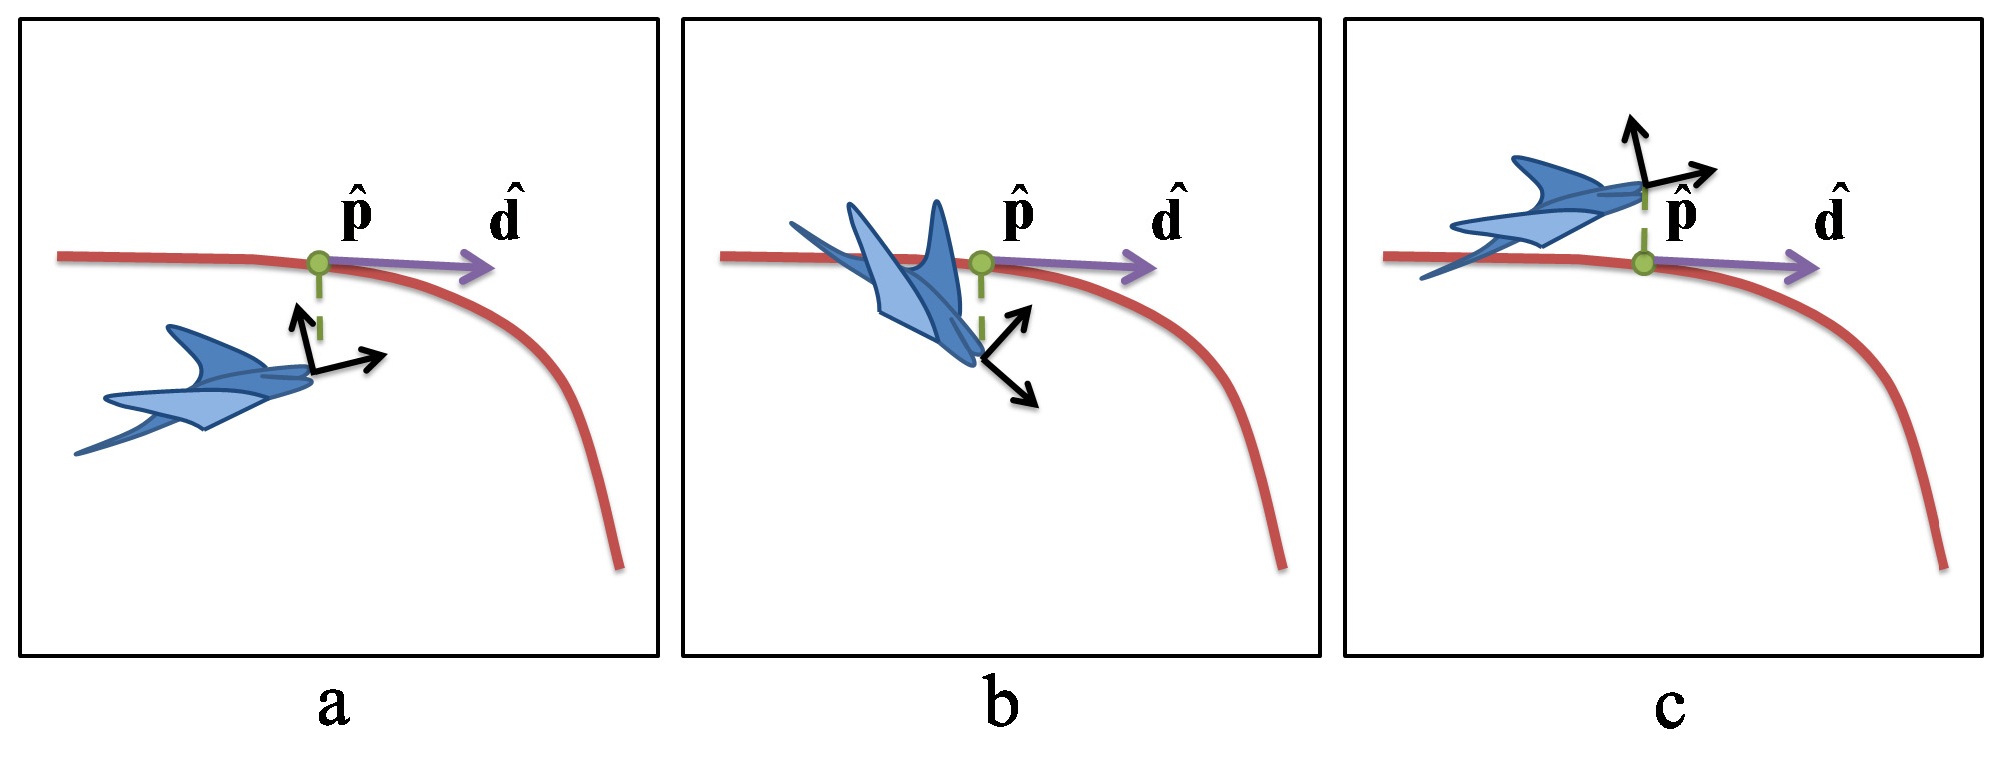
\includegraphics[width=3.2in]{figures/pathCase.eps}
\caption{Three different situations that determine if the creature chooses a ``swim straight'', ``pitch up'' or ``pitch down'' maneuver.}
\label{fig:pathCases}
\end{figure}

In addition to forward thrust, aquatic creatures also employ very
efficient turning maneuvers, such as pitching up and down or turning left
and right. The optimization technique described in Section
\ref{sec:optimization} can be modified to learn various
maneuvers. Once the aquatic creature builds a repertoire of swimming
maneuvers, we can combine different maneuvers to achieve a high-level
task such as path following.

First, we add another term to $E_{distance}$ in (\ref{eq:objFunc}) to maximize the turning angle towards the desired direction:
\begin{displaymath}
E_{distance}=\mathbf{d}^T(\Delta \mathbf{p})+\mathbf{r}^T(\Delta\mathbf{\alpha})
\end{displaymath}
where $\mathbf{r}$ is the desired axis of rotation. We set the desired swimming direction $\mathbf{d}$ half way from the current facing direction towards the turning direction. We also change $E_{deviation}$ to penalize the undesired orientation changes.
\begin{displaymath}
E_{deviation} = ||\Delta\mathbf{p}-\mathbf{d}^T(\Delta\mathbf{p})\mathbf{d}|| + ||\Delta\mathbf{\alpha}-\mathbf{r}^T(\Delta\mathbf{\alpha})\mathbf{r}||
\end{displaymath}
We solve the above optimization using the CMA method in the same way as described in Section 4.3.

Once different maneuvers have been learned, we apply a simple heuristic to
decide which maneuver to choose to follow the path. At the beginning of
each cycle of the motion, we find the nearest point $\mathbf{p}$ on the
path to the root of the articulated figure and transform $\mathbf{p}$ and
its tangential direction $\mathbf{d}$ to the root coordinate system. We
denote the transformed position and direction as $\hat{\mathbf{p}}$ and
$\hat{\mathbf{d}}$. Without loss of generality, let's consider a one
dimensional example. $\hat{p}_z$ is the z-component of $\hat{\mathbf{p}}$,
which means the point is above or beneath the root of the articulated
figure. Similarly, $\hat{d}_z$ indicates the path is going upwards or
downwards relative to the root orientation. We choose the different
maneuvers based on the following rules.
\begin{displaymath}
\textrm{Maneuver}=\left\{\begin{array}{ll}
\textrm{Go Straight} & \textrm{if } (\hat{p}_z \geq \epsilon \textrm{ and }\hat{d}_z \leq -\epsilon)\\
                     & \textrm{or } ( \hat{p}_z \leq -\epsilon \textrm{ and } \hat{d}_z \geq \epsilon)\\
\textrm{Pitch Up} & \textrm{if } \hat{p}_z > \epsilon \textrm{ and } \hat{d}_z > \epsilon\\
\textrm{Pitch Down} & \textrm{if }\hat{p}_z < -\epsilon \textrm{ and } \hat{d}_z < -\epsilon
\end{array}\right.
\end{displaymath}

\begin{figure}[!t]
\centering
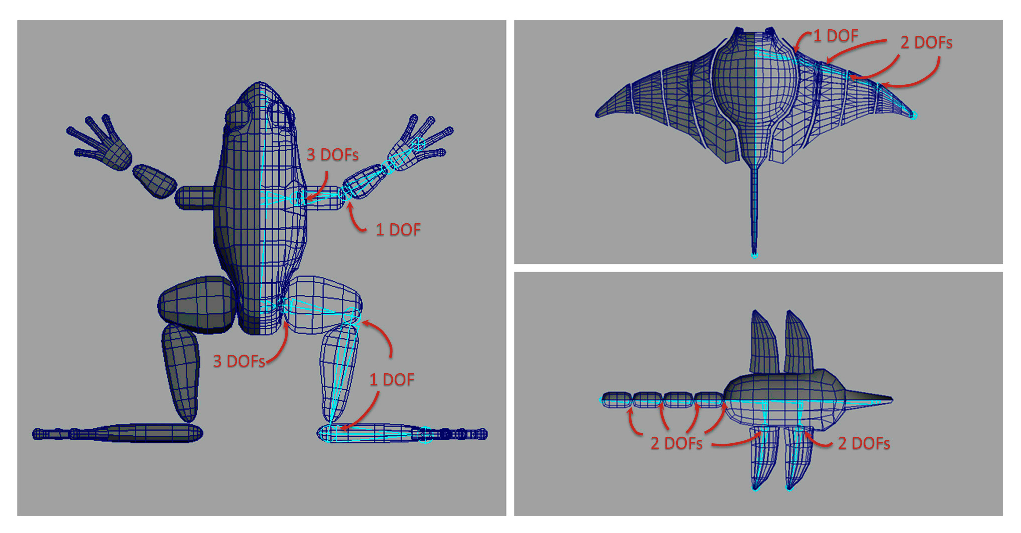
\includegraphics[width=3.2in]{figures/skels.eps}
\caption{The joint configurations of the frog, the manta ray and the alien.}
\label{fig:skels}
\end{figure}


\begin{figure}[!t]
\centering
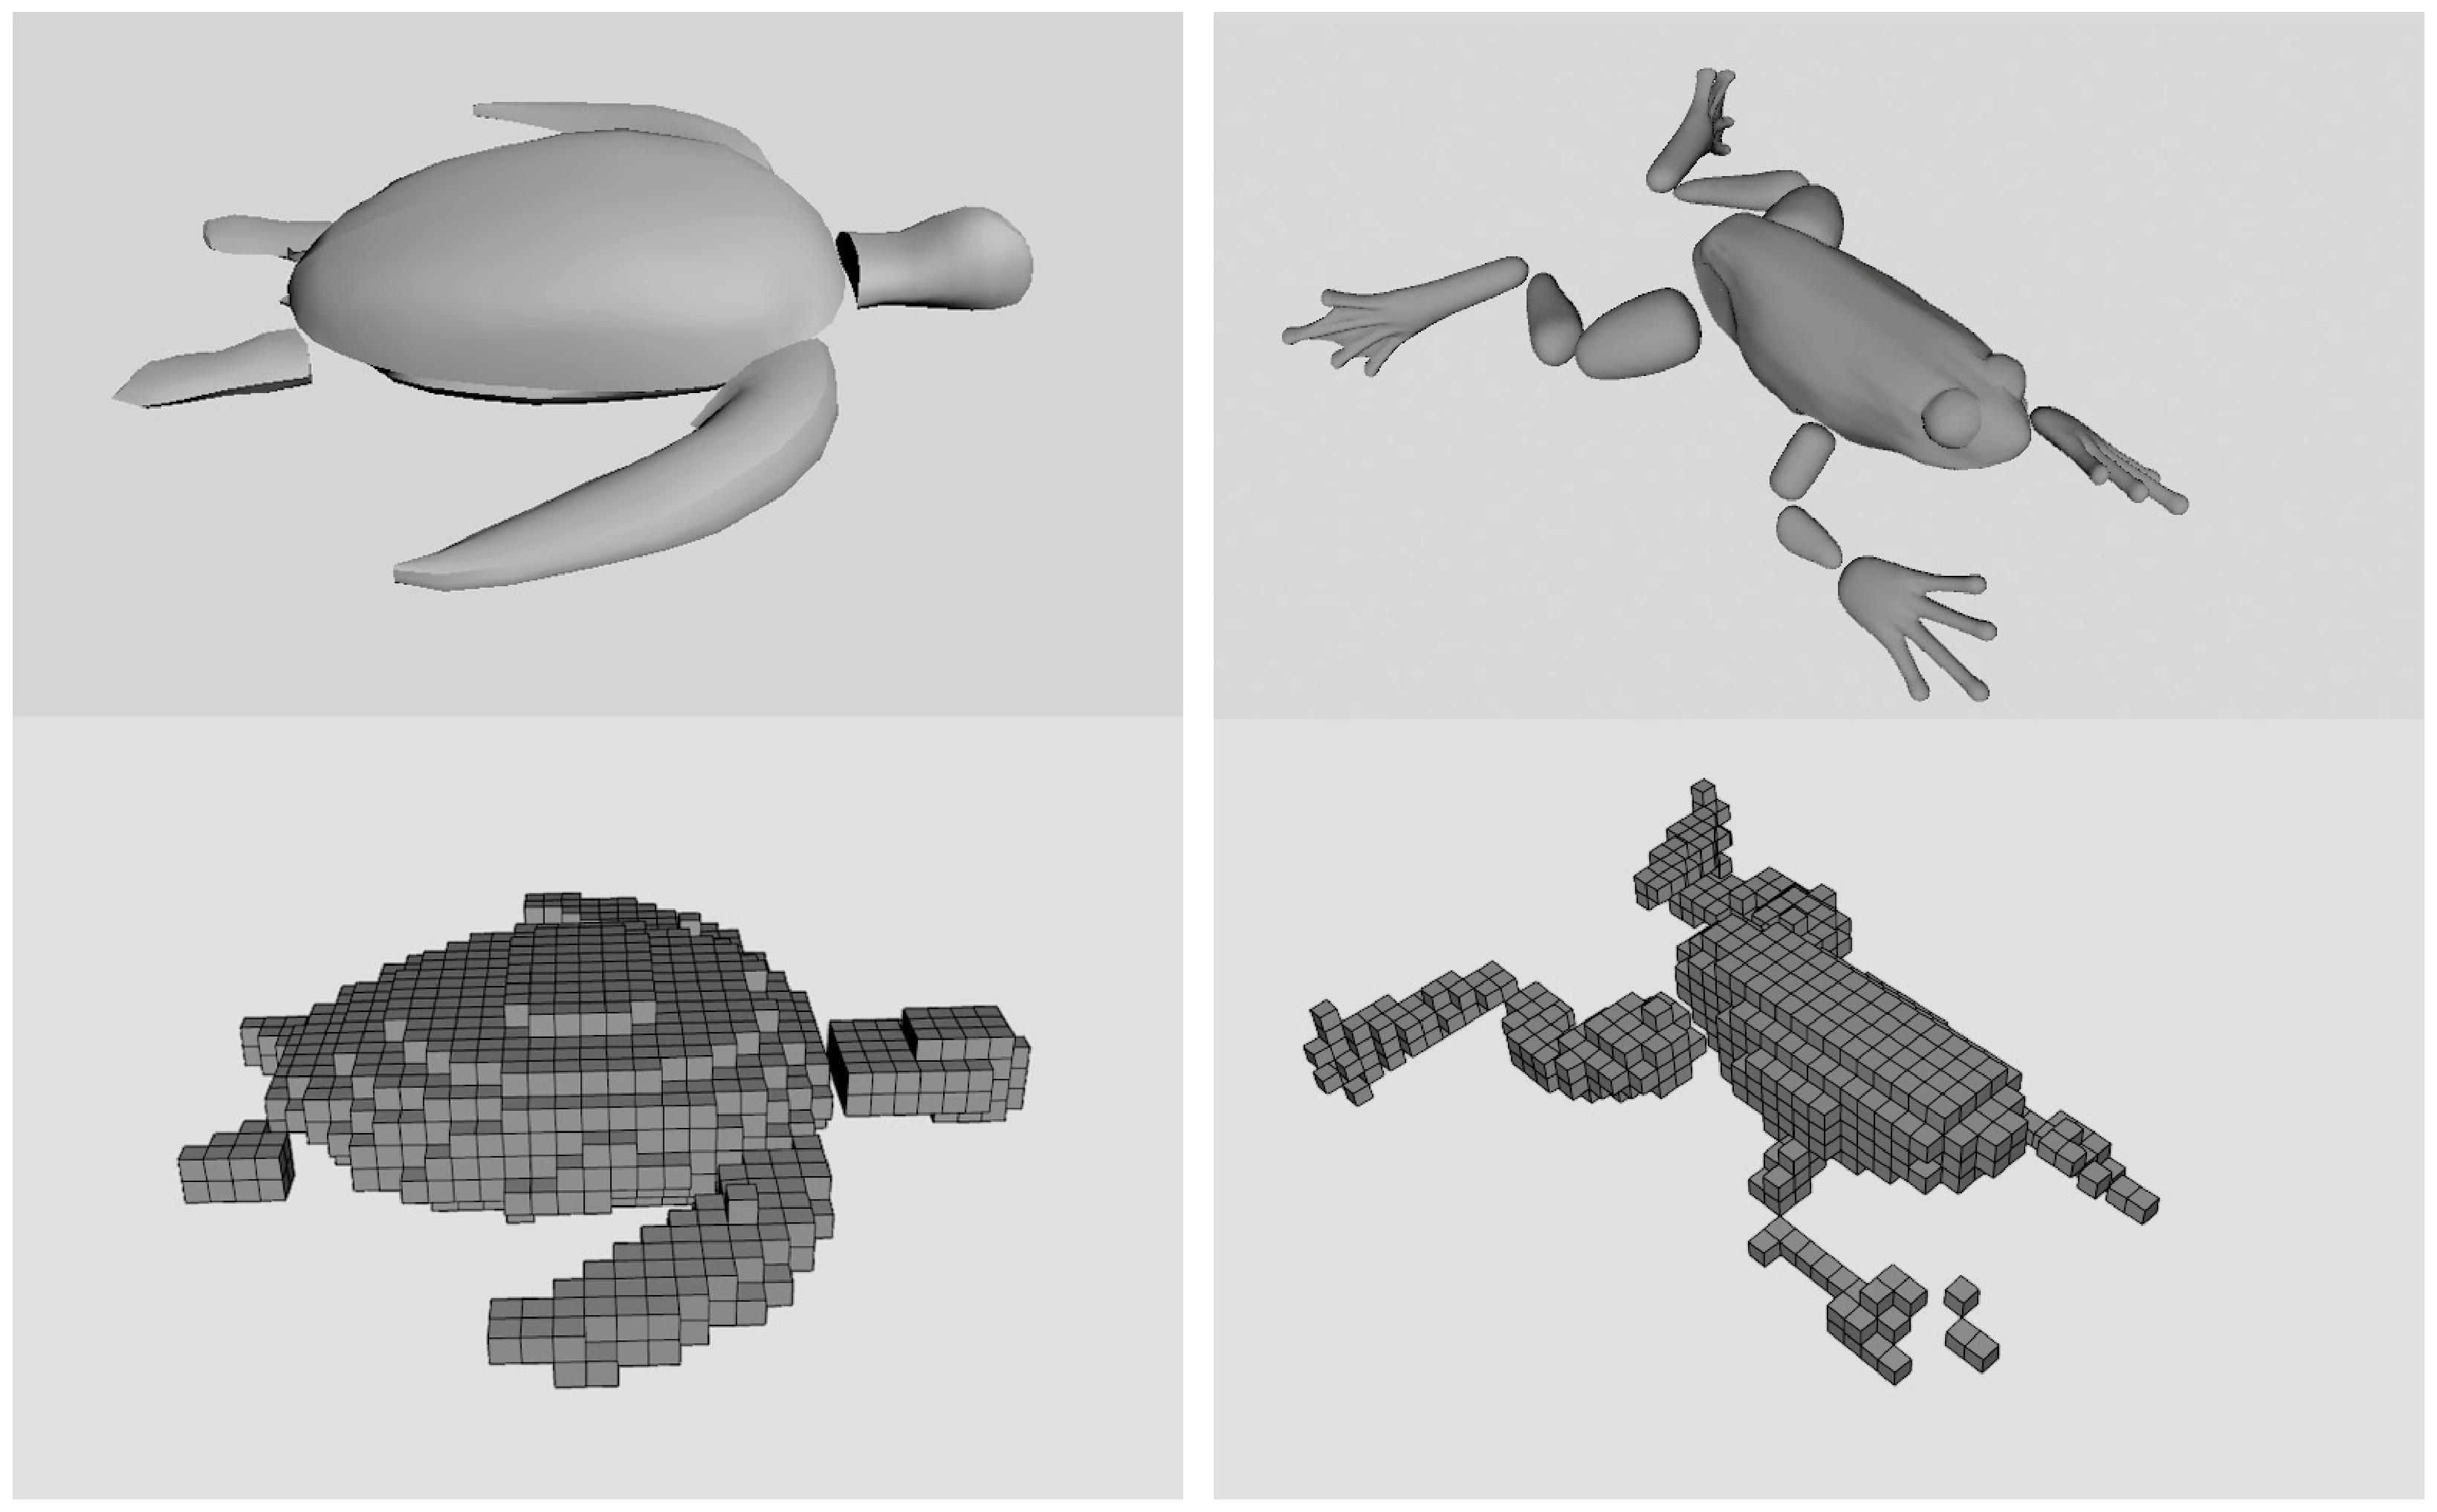
\includegraphics[width=3.2in]{figures/grid1.eps}
\caption{The voxelized representations of the turtle and the frog. The input shapes of the articulated creatures are represented by water-tight polygon meshes. We voxelize these body shapes onto the simulation grid each time step to simulate the two-way coupling between the fluid and the creature.}
\label{fig:grid}
\end{figure}

\begin{figure*}[ht]
\centering
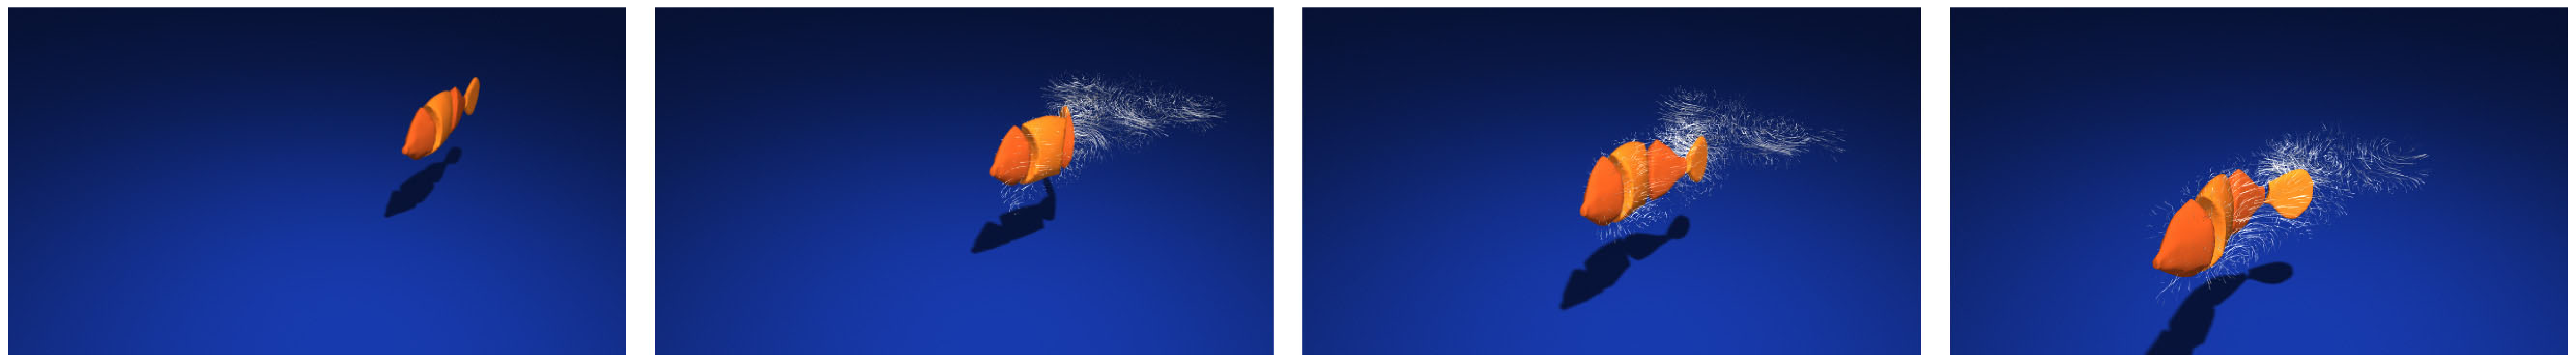
\includegraphics[width=\textwidth]{figures/fish.eps}
\caption{A four-link clown fish swims. Carangiform swimmers like this flex the front of their body a little, with the
majority of the motion near the tail. Note that this fish sheds two separate trails of vortices.}
\label{fig:fish}
\end{figure*}

\begin{figure*}[ht]
\centering
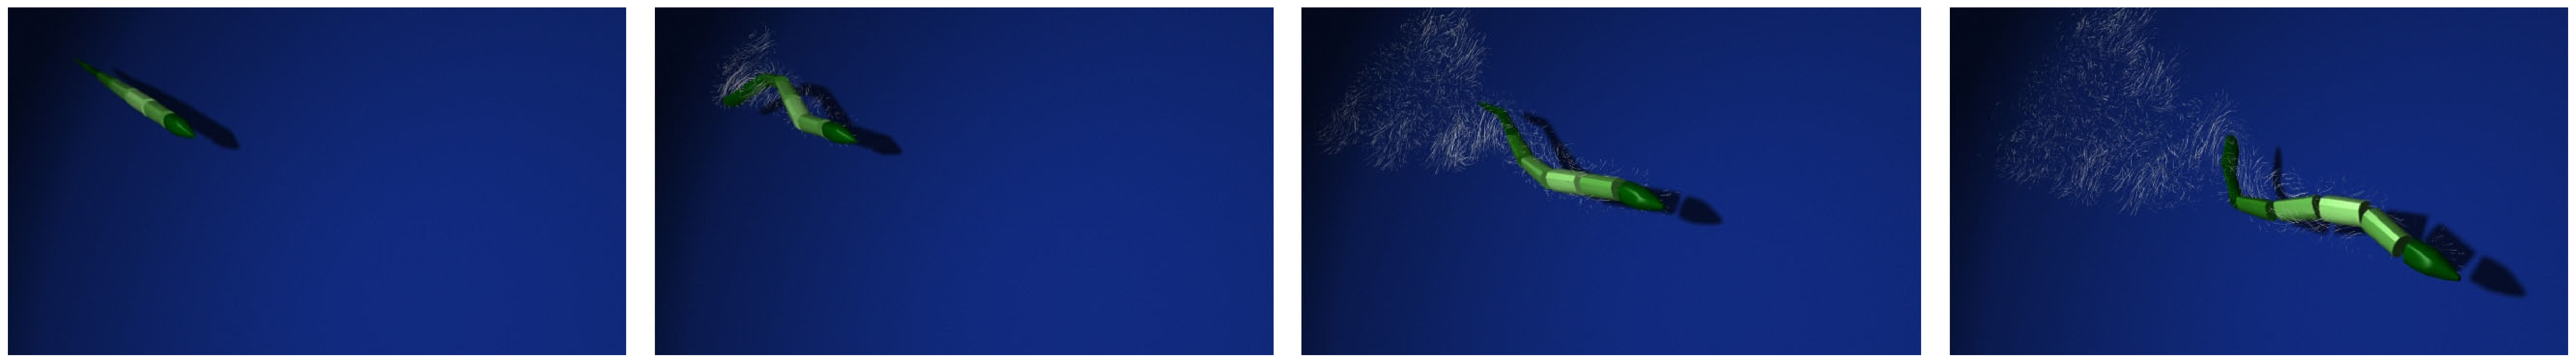
\includegraphics[width=\textwidth]{figures/eel.eps}
\caption{A swimming seven-link eel. Anguiliform swimmers undulate their whole body as if a wave is travelling from head to tail, and shed two separate trails of vortices from the tail.}
\label{fig:eel}
\end{figure*}

where $\epsilon$ is a small positive value to prevent the articulated
figure from repeatedly choosing alternating turning maneuvers due to small
deviations from the path. The first case indicates that the nearest point
on the path is above/below the articulated figure while the direction of
the path is going downwards/upwards. In other words, the articulated
figure is swimming towards the path (Figure~\ref{fig:pathCases}a). We
choose the action ``swim straight'' in this situation. On the other hand,
the second and third cases indicate the articulated figure is swimming
away from the path (Figure~\ref{fig:pathCases}b and \ref{fig:pathCases}c)
and we choose ``pitch up'' or ``pitch down'' accordingly.

\section{Results}

\begin{figure}[!b]
\centering
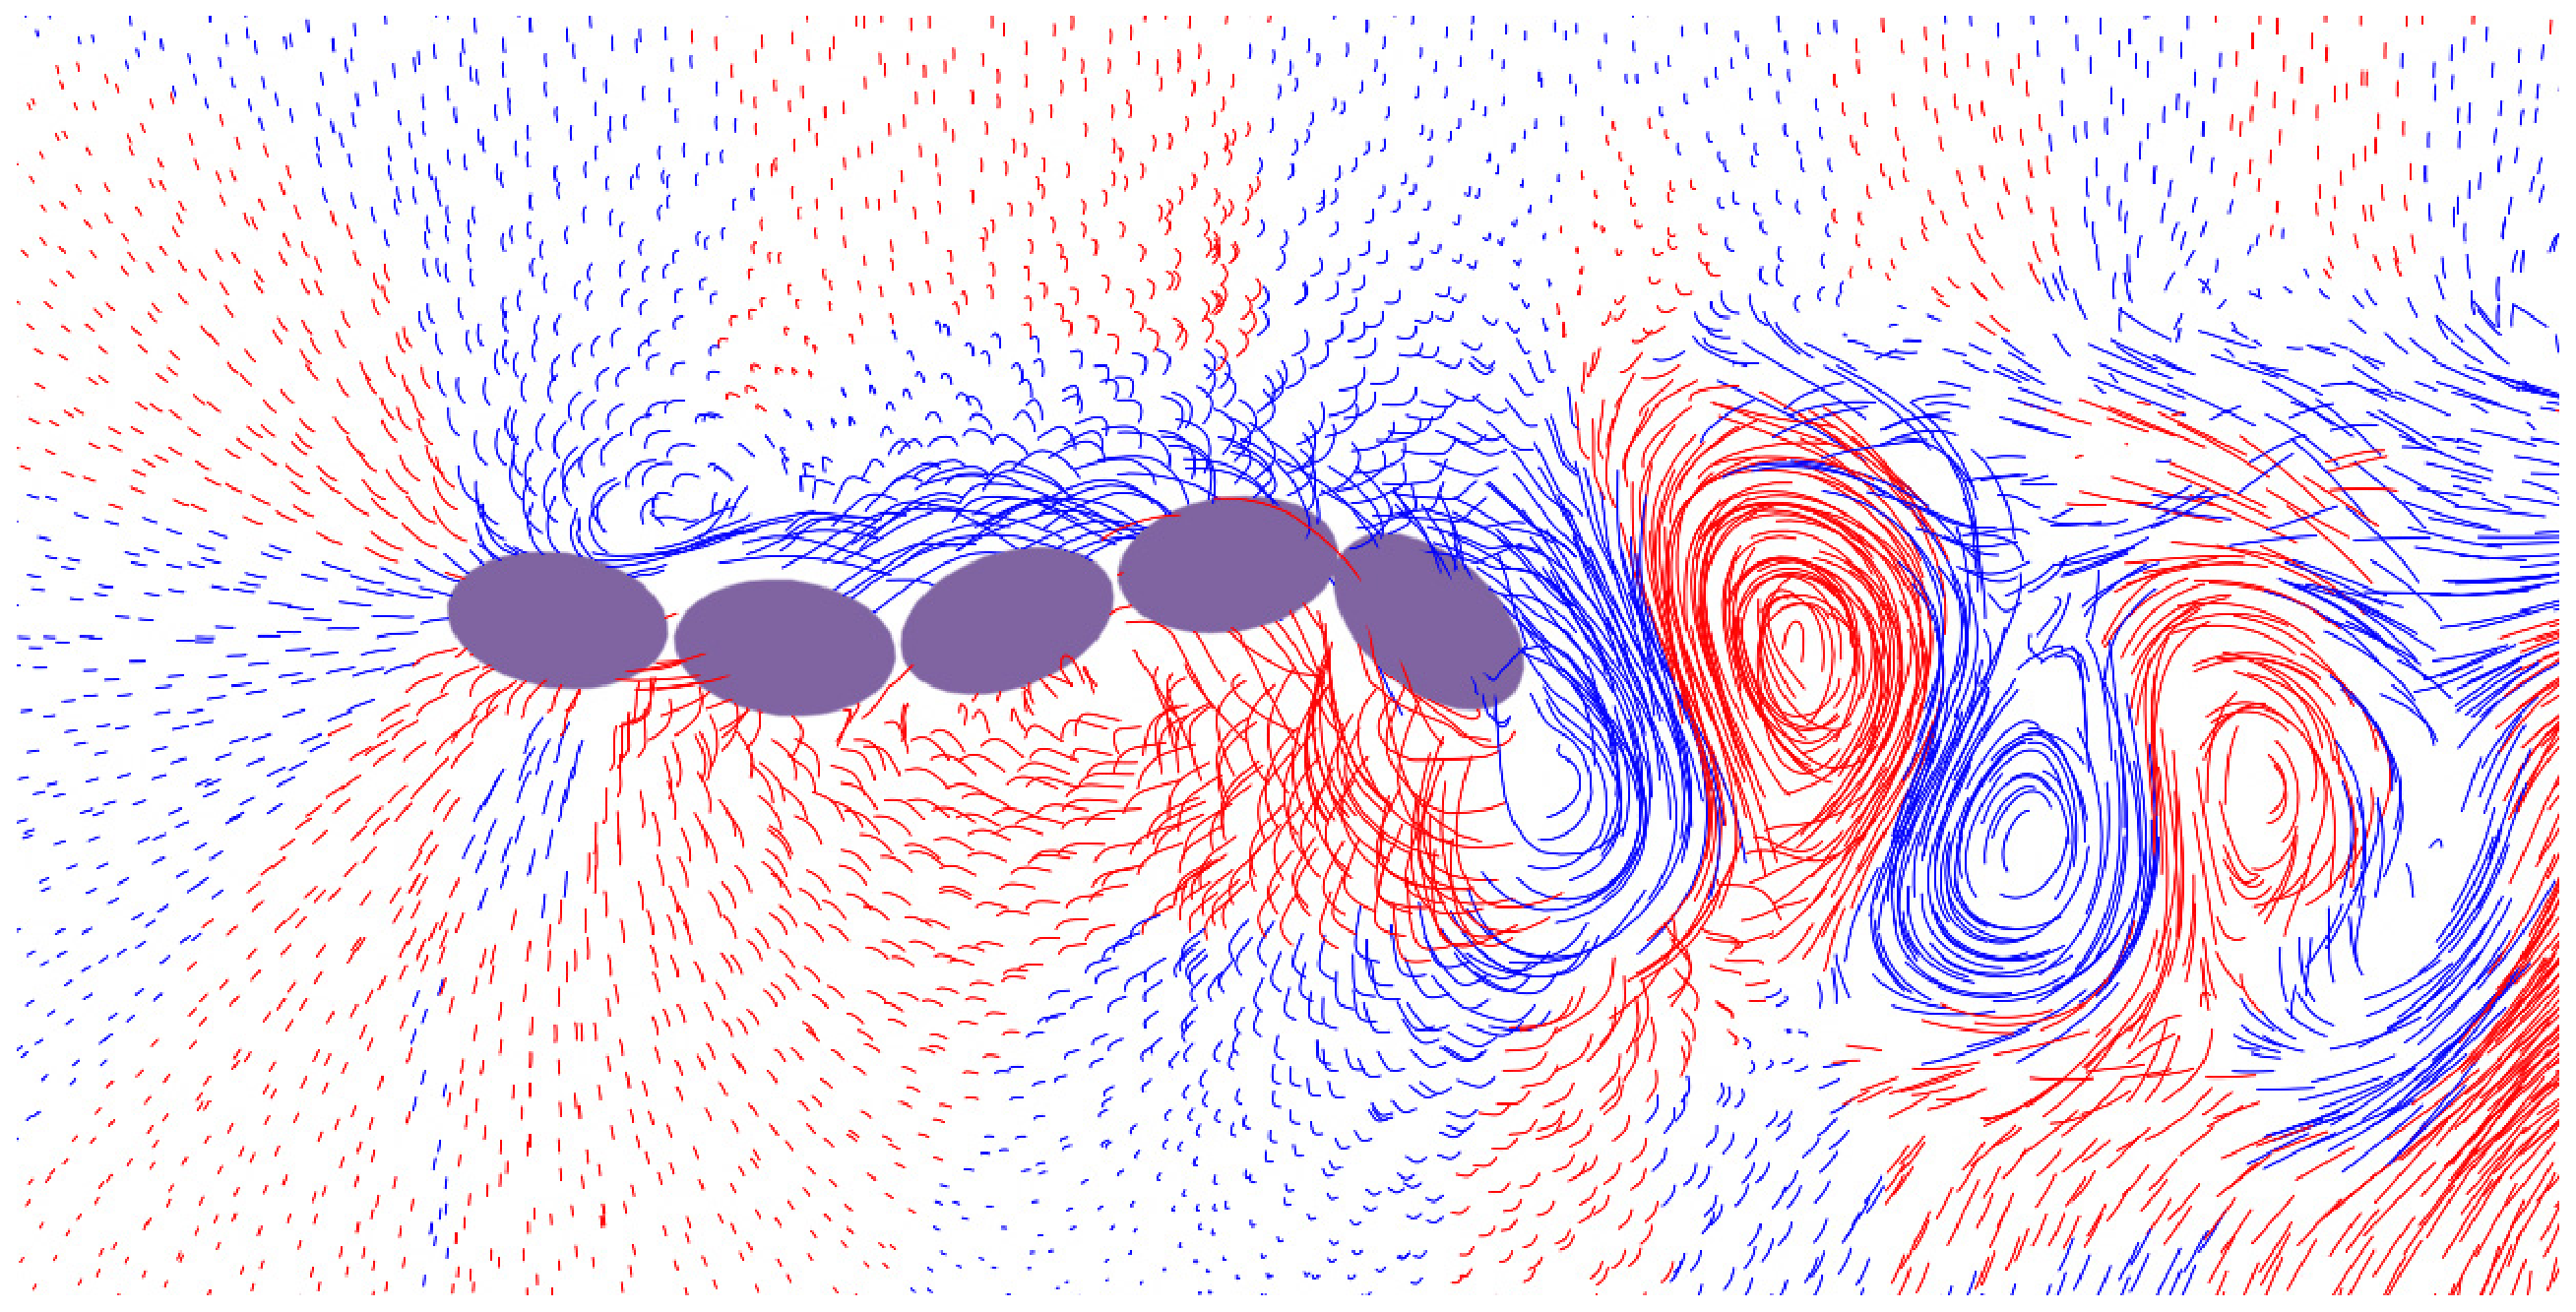
\includegraphics[width=3.2in]{figures/eel2D.eps}
\caption{A five-link eel swims in a 2D fluid environment. In contrast to the simulation in 3D, an eel swimming in 2D fluid sheds only one single vortex street. Red traces show the counter-clockwise vortices while blue traces show the clockwise vortices.}
\label{fig:eel2D}
\end{figure}

We implemented our method using C++ and ran CMA on a cluster with a
maximum of 100 iterations and with a population size of 16 for 2D and 31 for 3D
examples. Each CMA sample evaluates the objective function by simulating
two cycles of swimming motions. The optimization took from several hours
to two days, depending on the model and the grid resolution. After we
found the swimming gait, we ran the swimming simulation on a 2.26GHz CPU
with a single core.  All of the data for our swimming examples are
summarized in Table~\ref{table:simData}. In most of the cases, we use two
optimization variables, amplitude and phase, for each degree of freedom.
We set the period to one second and the offset to zero. When training the
turning gaits, we included the offset in the optimization variables. For the
accordian example, the degrees of freedom are interdependent and there is
no phase shift among the different degrees of freedom. Thus one
optimization variable is enough to characterize its motion. We also
exploited the strong symmetry in geometry for some creatures, such as
turtles and frogs, to halve the optimization dimensions. We illustrate the
joint configurations for some creatures in Figure~\ref{fig:skels} and the voxelized representations of creatures in Figure~\ref{fig:grid}.

\begin{table}
\centering
\begin{tabular}{|c|c|c|c|c|}
\hline
Examples & Num & Opt  & Sim  & Sim\\
         & DOFs & Dims & Res & Time \\
 \hline
accordian & 10 & 1 &  $120\times 80$           & 1.37s\\
eel(2D)   & 4  & 8 &  $128 \times 64$         &  0.64s \\
turtle(2D)& 4  & 4 & $64\times 64$           & 0.34s \\
fish      & 3  & 6  & $64\times 32\times 32$  & 1.45s\\
eel(3D)   & 6  & 12 &  $64\times 32\times 32$ & 1.31s\\
manta-ray & 14 & 21 &  $64\times 32\times 32$ & 10.92s\\
turtle(3D)& 10 & 10 &  $64\times 32\times 32$ & 11.29s\\
frog      & 18 & 18 &  $96\times 64\times 48$ & 12.79s\\
alien     & 16 & 24 &  $96\times 36\times 24$ & 10.75s\\

\hline
 \end{tabular}
 \caption{Parameters and performance of examples. Num DOFs is the number of degrees of freedom for the articulated rigid body. Opt Dims is the number of optimization variables. Sim Res is the grid resolution for the simulation and Sim Time is the average simulation time per frame.}
 \label{table:simData}
 \end{table}

In our implementation, we made three simplifications to reduce the
simulation cost. 1) Instead of using a large computational domain to cover
the whole space that the creature might swim to, we use a smaller domain
that is about two to four times larger in each dimension than the
creature's bounding box. This domain moves with the creature when the
creature approaches a boundary. 2) At the boundary of the computional
domain, we impose the Dirichlet boundary condition $p=0$ so that the fluid
outside the domain is free to flow in and vice versa. 3) Since the density
of most aquatic creatures is similar to that of the fluid, we ignore the force of gravity in our simulator.


\begin{figure*}[ht]
\centering
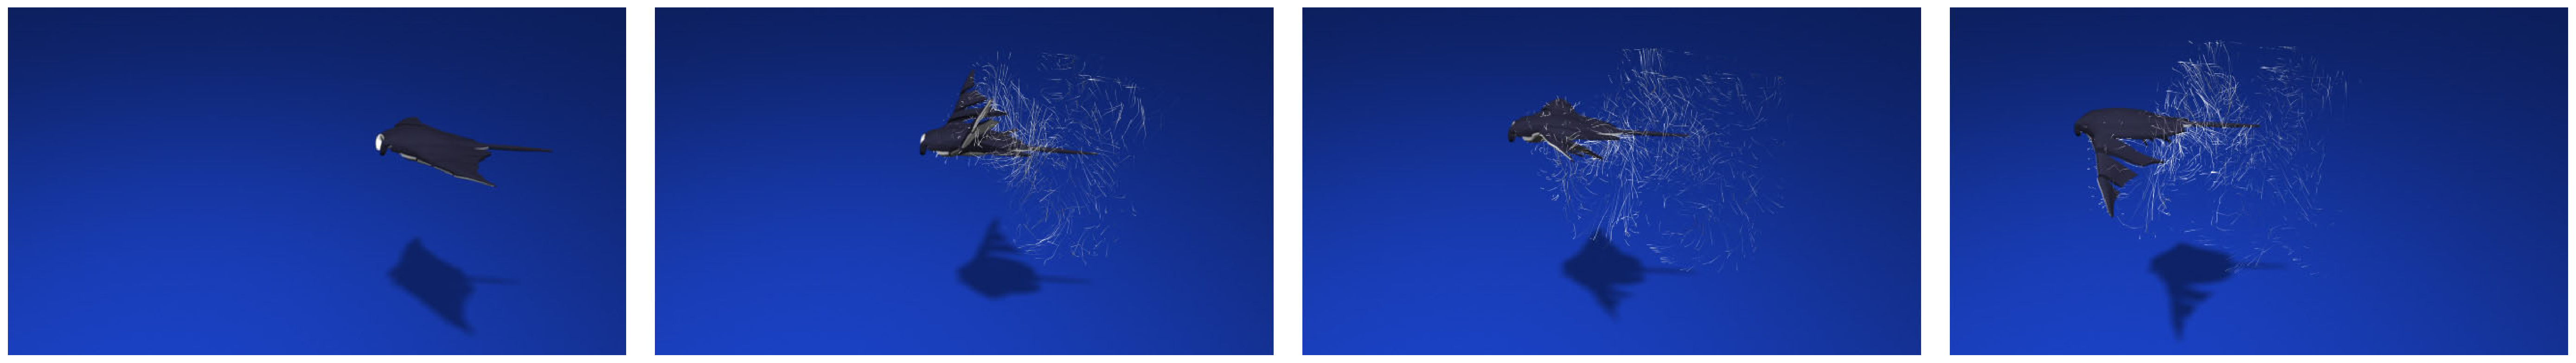
\includegraphics[width=\textwidth]{figures/manta.eps}
\caption{A manta ray swimming forward. Rajiform swimmers swim by slow flapping strokes like a slow-motion version of a bird flapping its wings.}
\label{fig:manta}
\end{figure*}

\begin{figure}[!b]
\centering
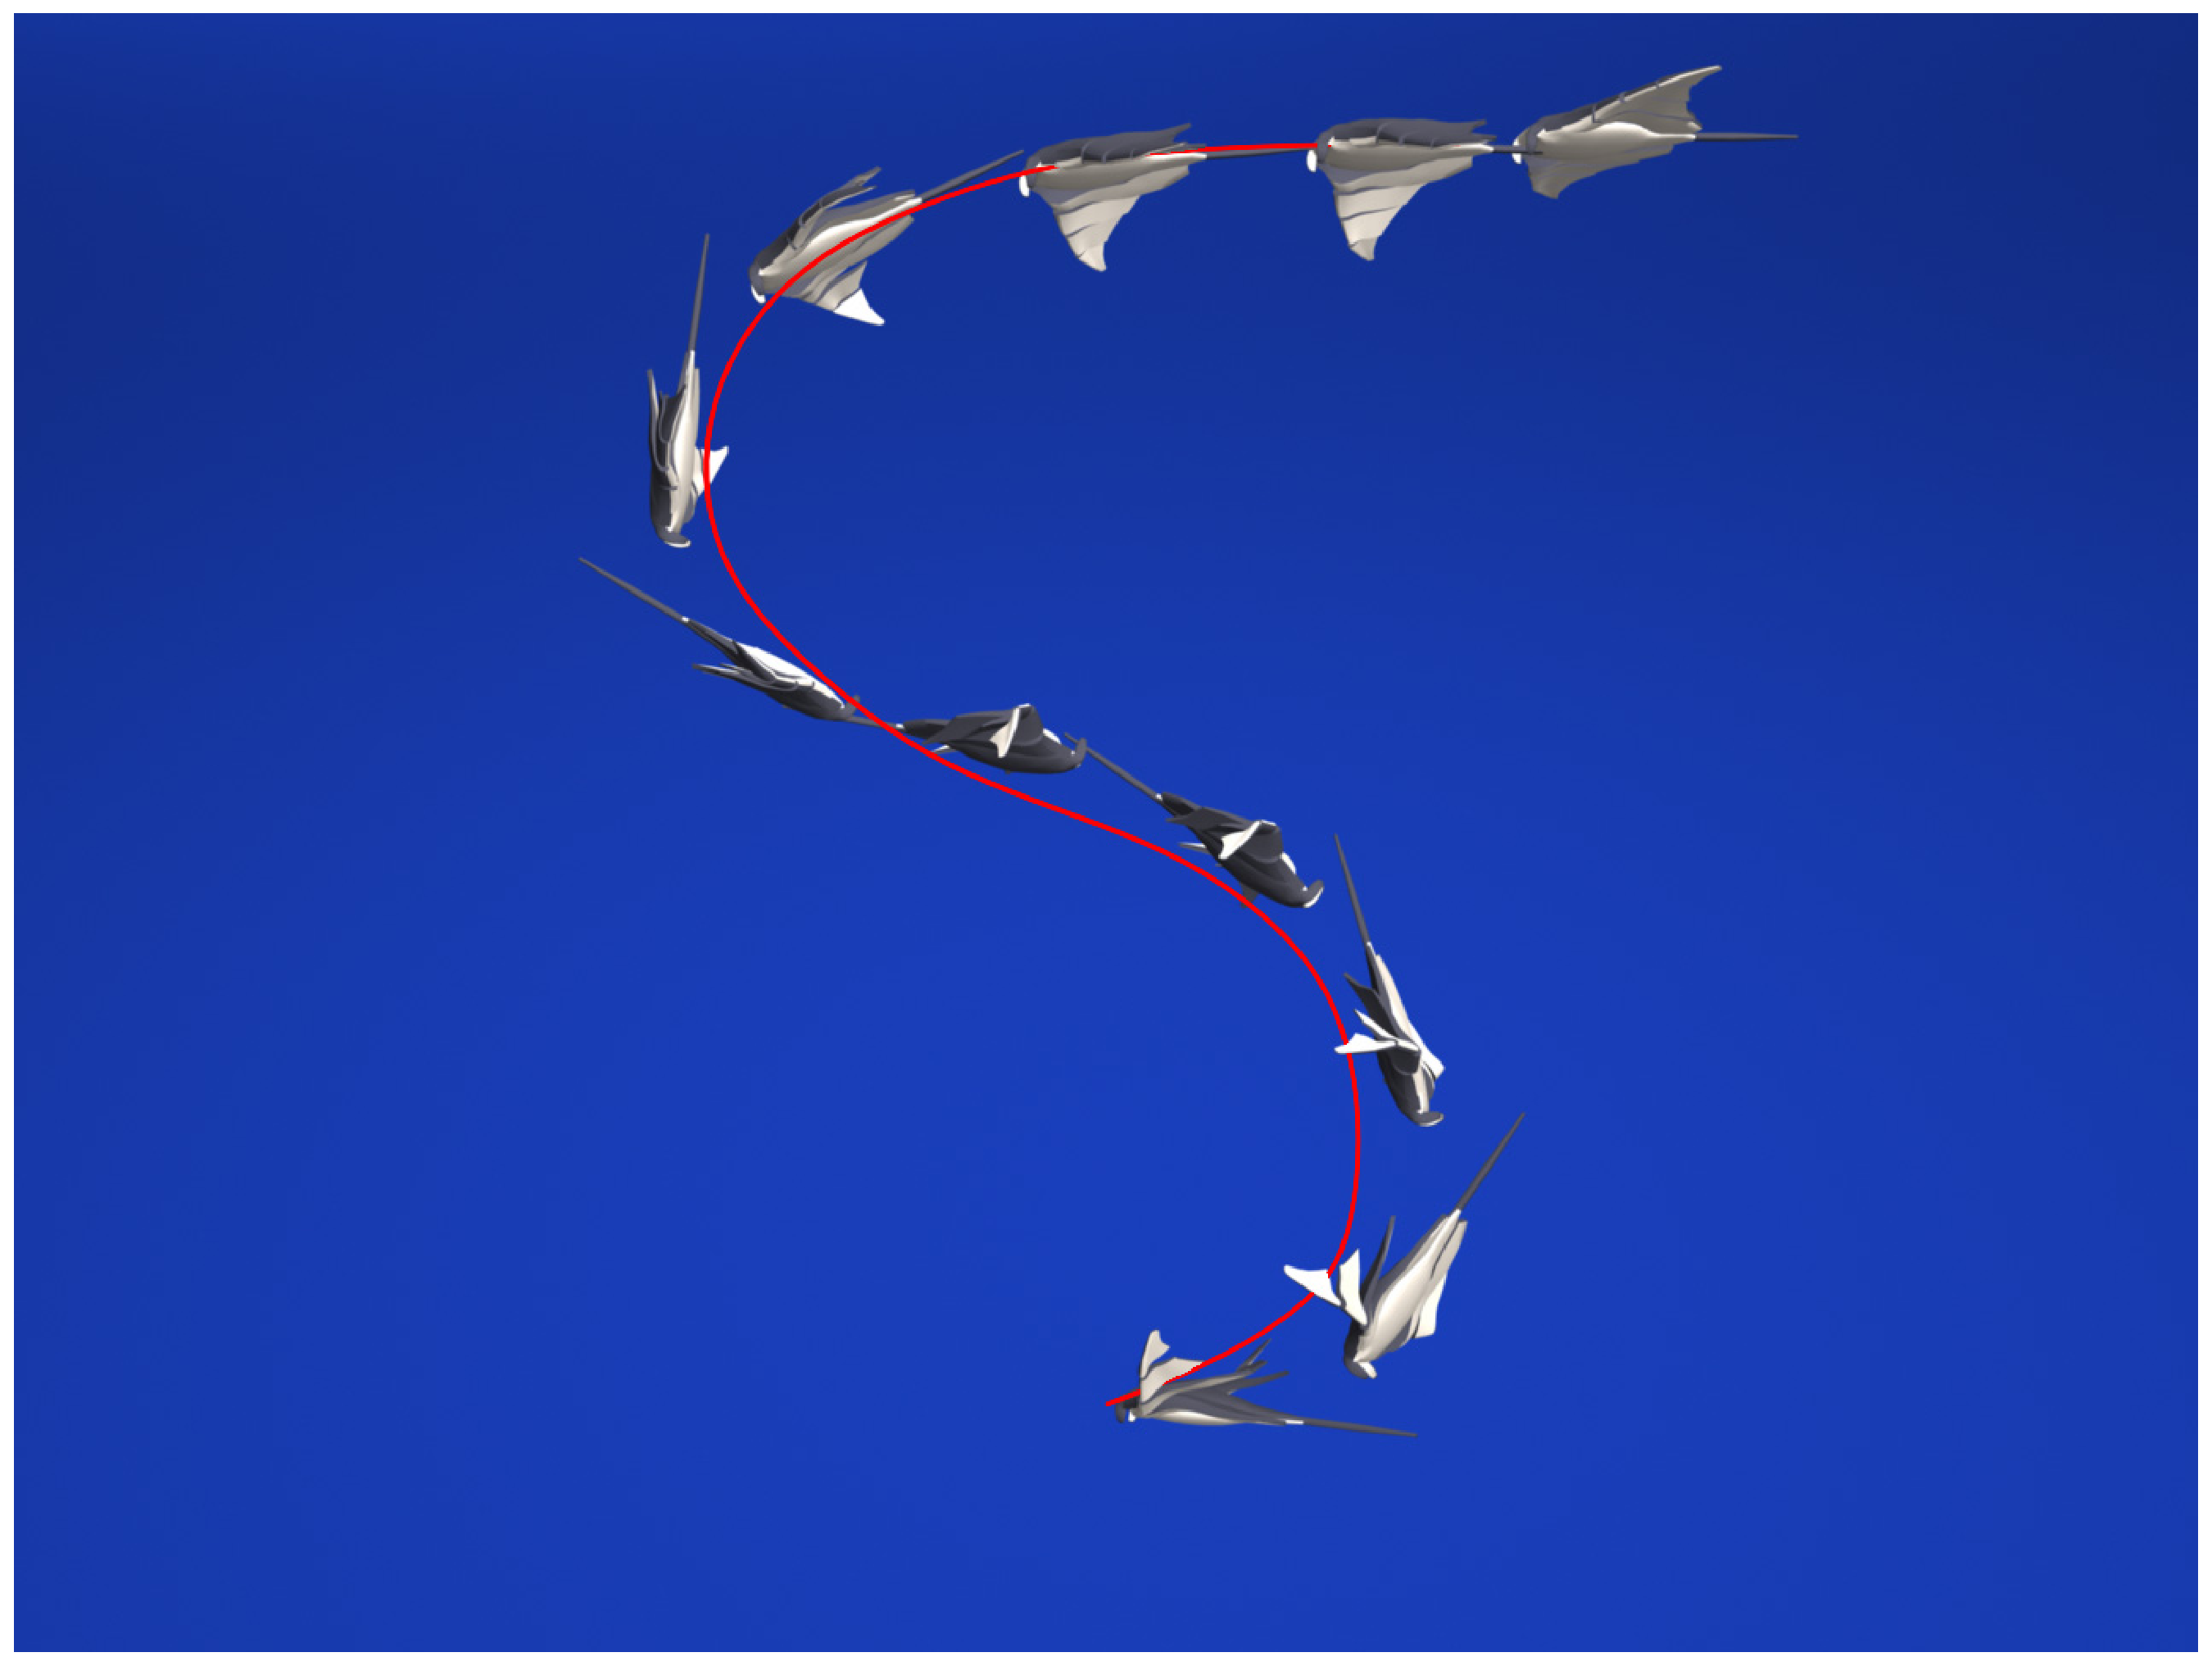
\includegraphics[width=3.2in]{figures/manta_path2.eps}
\caption{A manta ray follows an S-shaped path by choosing maneuvers from ``swimming straight'', ``pitch up'' and ``pitch down''. The red curve is the path specified by the user.}
\label{fig:manta_path}
\end{figure}

\begin{figure*}[ht]
\centering
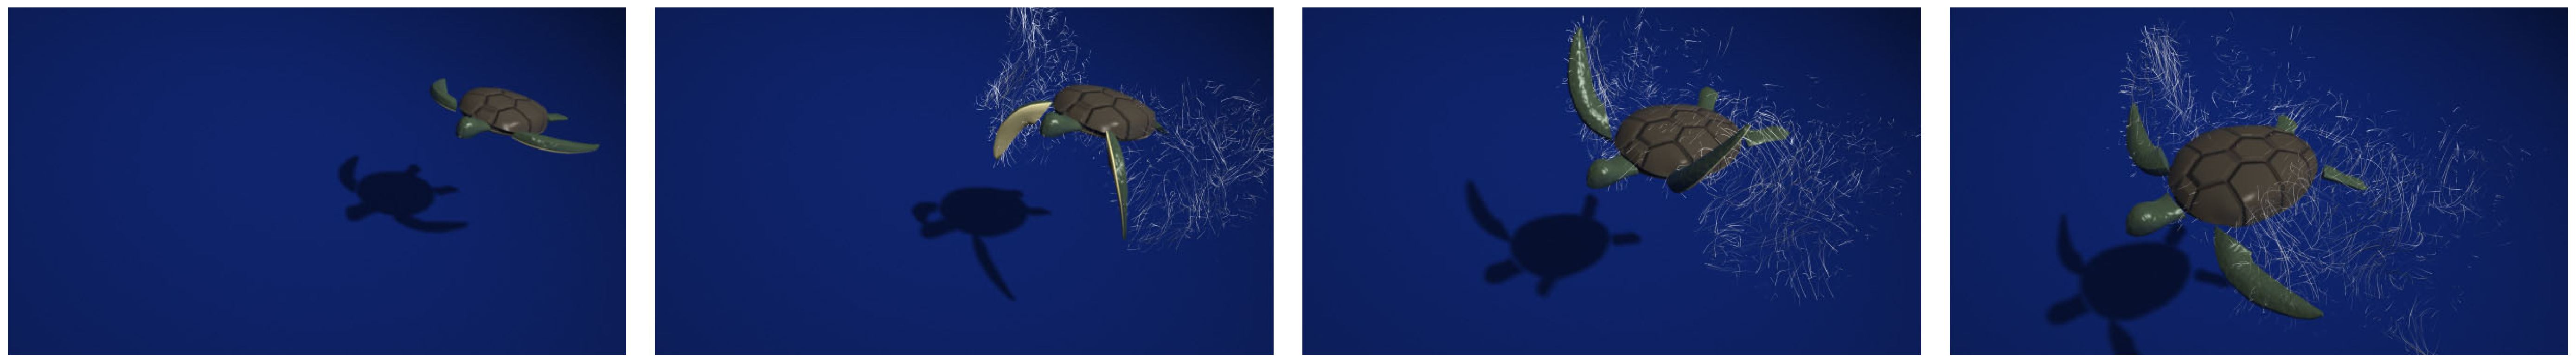
\includegraphics[width=\textwidth]{figures/turtle.eps}
\caption{A turtle swims in water with a flapping motion of its two front flippers. }
\label{fig:turtle}
\end{figure*}

We describe the results of our swimming optimization method.  Please see the video(http://www.cc.gatech.edu/~jtan34/project/videos/articulatedSwimmingCreatures.mp4) to observe the swimming
animations.  To visualize the fluid flow, we draw \emph{particles traces},
which show the trajectory of massless particles inside the fluid in a
short period of time (15 frames). We modulate the transparency of the
particle traces in 3D examples according to the magnitude of the vorticity
in order to focus attention on the visually interesting regions of the
flow.  In 2D examples, we colored the traces to indicate the directions of
the vortices.

\begin{figure*}[ht]
\centering
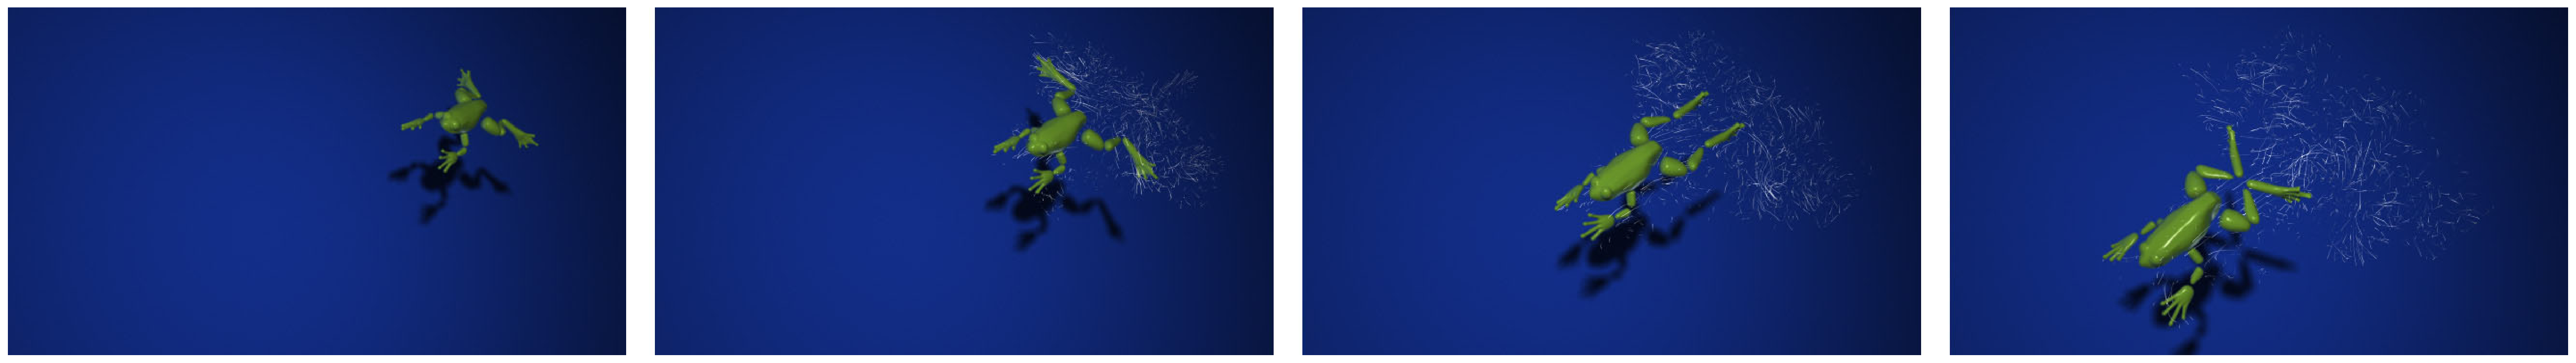
\includegraphics[width=\textwidth]{figures/frog.eps}
\caption{A frog mainly relies on its large rear legs to provide forward thrust in the water.}
\label{fig:frog}
\end{figure*}


\begin{figure*}[ht]
\centering
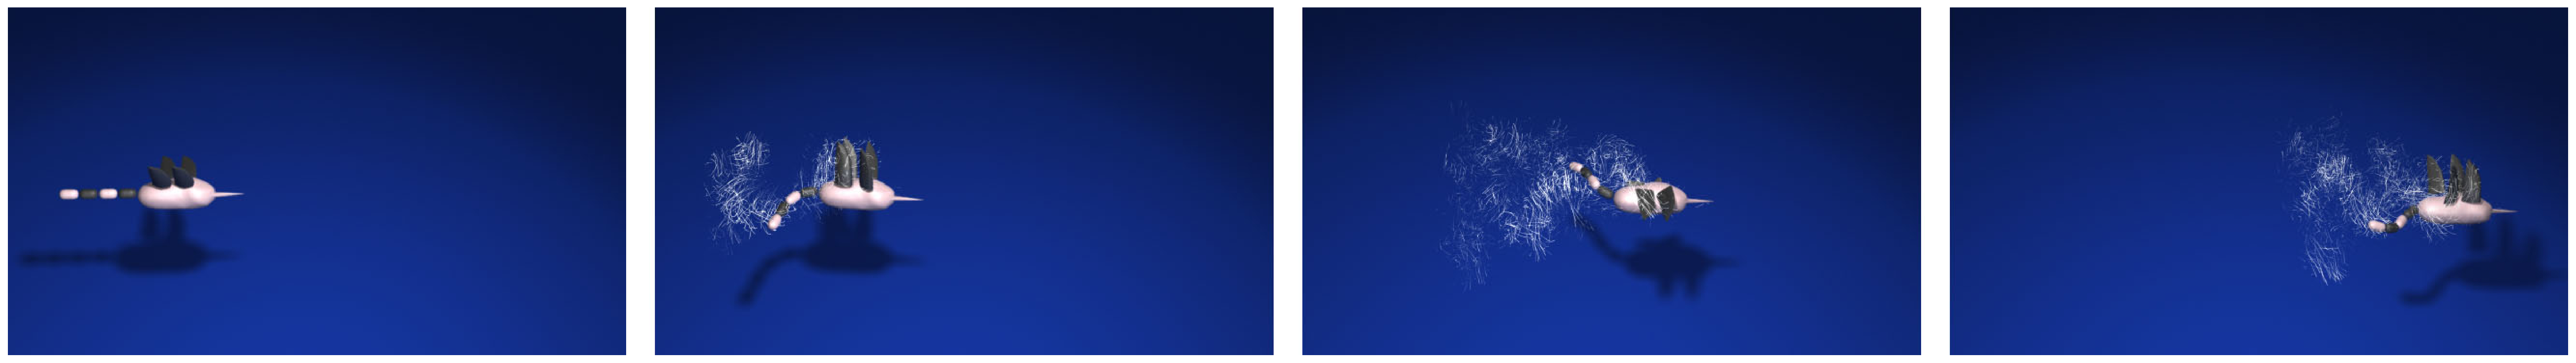
\includegraphics[width=\textwidth]{figures/alien.eps}
\caption{An alien aquatic creature that swims in water by undulating its tails and flapping its wings. Note the two pairs of wings are slightly out of phase to mimic flapping motion of larger wings.}
\label{fig:alien}
\end{figure*}



There are many body shapes and styles of locomotion for fish, and our
first set of results investigates several of these.  Figure~\ref{fig:fish}
shows a four-segment model of a fish, modelled after the body shape of the
clownfish.  We used CMA to optimize for efficient forward motion, and snapshots of the resulting motion are given in the figure.  Note that the
forward body flexes just a little, with the majority of the motion near
the tail, which is in good agreement for the style of motion known as the
carangiform mode~\cite{lindsey1978form}.  Using the same objective
function, we optimized a seven-segment figure that was designed to mimic
an eel body.  Figure~\ref{fig:eel} shows that the resulting motion is that
of a travelling wave along the body of the creature, as is typical of real
eel swimming (anguiliform mode).  Note that the wake of our eel has two
separate trails of vortices that are shed from the tip of the tail, as has
been observed in lab studies of eels~\cite{tytell2004hydrodynamics}. We show in Figure~\ref{fig:eel2D} that a different wake structure appears when an eel swims in a 2D fluid environment, that of a single vortex street. The difference of the wake structure between the 2D and 3D simulations agrees with Kern and Koumoutsakos's study of eels \cite{kern2006simulations}.


Our final example of fish motion is that of a manta ray.  The manta has a
body that is thin in the vertical direction and that has large pectoral fins
that extend in the horizontal direction.  It swims by slow flapping strokes
of these wing-like pectoral fins (the rajiform swimming mode), somewhat like
a slow-motion version of a bird flapping its wings.  Although the manta ray
does not seem to be a good candidate to be modelled as an articulated
figure, we wanted to see how far the articulated models could be pushed.  We
modelled the ray's pectoral fins as four rows of thin plates that are
connected to one another near the leading edge of the fin.  The resulting
swimming motion from the optimization procedure exceeded our expectations,
producing the same graceful flapping that these creatures use to swim (see
Figure~\ref{fig:manta}).

We tested our path following approach using the manta ray model.  We used
our optimization method to find efficient swimming for forward motion, an
upward turn and a downward turn.  We then gave the manta ray a vertical
S-shaped path to follow using our path following controller.  The
simulated ray was able to follow the path quite closely, as the composite
image in Figure~\ref{fig:manta_path} shows.  Note that this path following
motion was created with a single simulation, based on gait switching
between the three learned basic motions. We also tested the path following
algorithm using a simple 2D turtle model. We show that the turtle cannot
swim straight without using the path following technique due to the
accumulation of numerical errors. When the path following technique is
applied, the turtle actively adjusts its swimming motions according to its
position and orientation and successfully swims straight.

Figure~\ref{fig:turtle} shows the motion of a sea turtle that was created
using optimization.  Adult sea turtles are underwater fliers, moving
themselves forward with a flapping motion of their two front flippers that
is called a \emph{powerstroke}~\cite{wyneken1997}.  Note that our turtle
results show the characteristic rotating of the front flippers during the
upward stroke.  Figure~\ref{fig:frog} shows the results of our swimmer
optimization for a model frog.  As with real frogs, the large rear legs
provide the forward thrust using a classic frog kick. Note that the frog uses its forelimbs with a small range of motion. We think this is because the contribution from the arms is small relative to the contribution from the legs. Based on our observation, some real frogs do not use their forelimbs much when swimming.

In the accompanying video, we also demonstrates that articulated figures
can differ dramatically in their swimming motion depending on whether the
simulated fluid is a simple model or a full Navier-Stokes (NS) solver.
Our simple fluid simulator calculates the force as the square of the
normal component of the velocity of a moving surface element.  This
simplified fluid model is identical to that
in~\cite{wu2003realistic,lentine2010creature}.  We show that swimming in
different fluid models leads to different locomotions. Figure~\ref{fig:accordian} shows a 2D swimmer that
compresses and relaxes its body in an accordian-like manner moves through
the water in the NS fluid but stay in one place in the simple fluid. We
demonstrate that the gaits trained in different fluid models differ
considerably.  The swimming gait for a fish trained in NS fluid smoothly
flaps its tail to propel itself forward.  When this same fish model is
optimized using the simple fluid, the resulting motion is considerably
different, gaining thrust mainly from bending at a sharp angle at the
middle joint of the body.  These differences in motion between a simple
fluid and the NS fluid are in agreement with the findings of Lentine et
al.~\cite{lentine2010creature}.

In order to test the generality of our method, we applied our swimming
optimization to an articulated figure that has no counterpart in the real
world (see Figure~\ref{fig:alien}).  This is the swimming version of the task of finding plausible walking
motions for a user-created land
creature~\cite{hecker2008real,wampler2009optimal}.  Our alien creature has two
pairs of limbs on the trunk of its body, and in addition has a long and
powerful tail.  The motion that was found by our optimization combines a
whip-like motion of the tail together with coordinated rowing from the pairs of
limbs.  Although there is no point of comparison in the real world for this
creature's motion, the resulting swimming pattern looks entirely plausible.

\begin{figure}[!b]
\centering
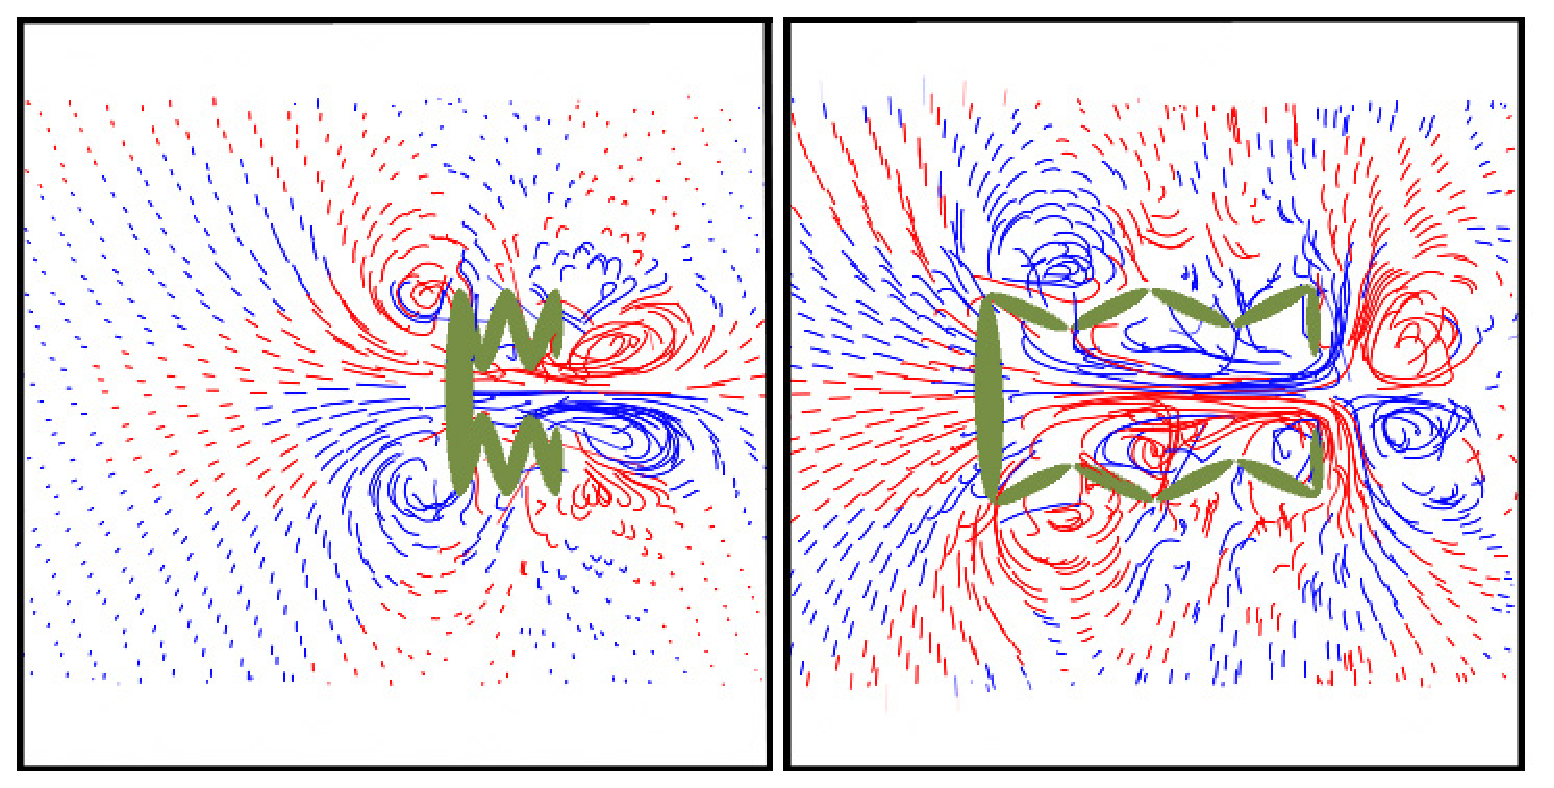
\includegraphics[width=3.2in]{figures/accordian.eps}
\caption{An imaginary creature swims forward by compressing and relaxing its body in an accordion-like manner in a Navier-Stokes fluid model. The images are two snapshots in the animation sequence. This demonstrates that including the Navier-Stokes fluid model is necessary to capture certain swimming patterns, such as jet propulsion, because a simplified fluid model does not allow forward motion for such modes of locomotion.}
\label{fig:accordian}
\end{figure}

Although our method requires little prior knowledge about the swimming gait of the creature,
there are some parameters that users can change, including the energy bound, the period of
the motion for each degree of freedom, and joint limits. This provides users the freedom to
achieve different motion, agile or slow, by changing these parameters. In particular, we tuned the period
of the swimming gait and the energy bound in our examples. We used a period of one second
for all of the examples. We made this choice deliberately because choosing a longer period means longer
optimization time (each CMA sample need to simulate two cycles of swimming motions). However, we believe
that including the period into the optimization will probably give more interesting results because different periods could make
a big difference in the final swimming gait. We leave this as future work. To set the energy bounds, we began by trying out several energy bounds
for an initial animal, the fish shown in the upper left of Figure~\ref{fig:teaser1}.
Once we were satisfied with the results, we then used this as our standard energy bound.
For a new creature, we scaled this standard energy bound according to the mass of the new creature
relative to the mass of the fish. Users can also change the weights in the objective function.
In our examples, we set all these parameters by intuition without much tuning. The weights
are reported at the end of each paragraph that introduces the different objectives in Section 4.2.

\section{Discussion}

We have demonstrated that our approach creates natural swimming behavior for
a wide variety of animal bodies.  For short-bodied fish and eels, our
results show vortex trails that are in agreement with laboratory
measurements and other published simulation results.  For the other
creatures, our optimized motions have the same overall appearance of the
real-world animals, although lab data is not available.  Our articulated
body representation of creature anatomy is quite general, even allowing us to
animate forms such as the manta ray that are not usually thought of as
articulated figures.

Although we have successfully applied our method to various aquatic
creatures with disparate body shapes and joint configurations, our approach does
have limitations. Our two-way coupling method needs to voxelize the articulated rigid body,
and the accuracy for representing the articulated figure depends on the grid
resolution. Thin features cannot be captured by the fluid simulator (Figure~\ref{fig:grid}). We believe that incorporating adaptive grids
\cite{Losasso04Octree} or unstructured meshes
\cite{Brochu10MatchingElement,klingner2006mesh} can dramatically increase
the accuracy of the two-way coupling. Furthermore, the two-way coupling
method is tailored for the interaction between fluids and articulated
figures. Even though many aquatic creatures have a skeleton and can be
represented well by articulated figures, there are exceptions such as
jellyfish. Our framework for discovering the optimal swimming gaits and
path following is still valid for soft-body creatures, but we would need
an efficient two-way coupling mechanism to simulate these swimming
motions. We leave this as future work.

We use the sine function to parameterize the joint space. There
are quite a few motions that cannot be depicted by a single sine function,
such as gliding. One possible way to improve this is to to use a weighted
sum of multiple sine functions with different amplitudes, phases and
periods \cite{Grzeszczuk95automatedlearning}. However, this would require more
optimization variables and more computational resources to discover a
swimming gait.

Our simulated swimmers seem to use more energy than the real creatures do because the simulated water is more viscous than real water. Even though we use the inviscous Navier-Stokes equation (Euler equation) to simulate the fluid, there is numerical viscosity. We chose to use relatively coarse grid, and thus incur large numerical viscosity, to keep the computational time tractable because CMA optimization need to simulate the two-way coupling thousands of times. In addition, while the real aquatic creatures take advantage of their streamline shaped body to reduce the fluid drag, the simulated creatures are voxelized and the resultant stair-step shaped body is not particularly efficient inside the fluid.

There are a number of interesting avenues for future work.  There are many
ways this approach could be expanded to give more control to animators,
including different path following strategies and higher-level behavior
control.  Our work has concentrated on continuous motion, but many animals
have distinctly different movements for situations such as escaping a
predator.  It would be interesting to investigate these faster, intermittent
motions.  Swimming at the \emph{surface} of the water could be studied,
including motions such as a human swimmer doing the crawl or a whale jumping
out of the water (breaching).  Finally, taking a cue from the work of Karl
Sims, it would be fascinating to simultaneously optimize for both swimming
motion and body shape.
